\documentclass[a4paper,11pt]{report} % Can add twoside for even/odd margins

%\usepackage{UmUThesis}           % Standard English
\usepackage[noindent]{UmUThesis}  % Non indented English
%\usepackage[se]{UmUThesis}       % Swedish

\usepackage[utf8]{inputenc}
\usepackage{courier}              % Nicer fonts are used. (not necessary)
\usepackage{pslatex}              % Also nicer fonts. (not necessary)
%\usepackage{lmodern}             % Optional fonts. (not necessary)

\usepackage{hyperref}
\usepackage{url}
\usepackage{xurl}
\usepackage{hyphenat}
\usepackage{siunitx}

\usepackage{booktabs}
\usepackage{tabularx}
\usepackage{array}
\usepackage{float}
\usepackage{graphicx}

\usepackage[capitalise,noabbrev]{cleveref}
\usepackage[nohyperlinks]{acronym} 
\usepackage{comment}

\hypersetup{
    colorlinks=true,
    linkcolor=black,
    filecolor=magenta,
    urlcolor=blue,
    citecolor=black,
}

\emergencystretch=2em
\newcolumntype{R}{>{\raggedleft\arraybackslash}X}
\newcolumntype{L}{>{\raggedright\arraybackslash}X}
\newcolumntype{Q}[1]{>{\raggedright\arraybackslash}p{#1}}

\title{Monthly Electricity Consumption Forecasting Using an Explainable AI Framework}
%\subtitle{If you have a subtitle}
\author{Tyra Wodén}
\supervisor{Esteban Guerrero Rosero} % Supervisor at UMU
\supervisore{Elin Eriksson} % External supervisor
\examiner{Ola Ringdahl} % Examiner
\semester{Spring 2026}
\course{Degree Project in Interaction Technology and Design, 30 credits}
\education{Master of Science Programme in Interaction Technology and Design, 300 credits}

\graphicspath{{pictures/}}

\pagestyle{empty}

\begin{document}
\maketitle

\cleardoublepage


\begin{abstract}
    %An abstract is a short description (10-20 lines) of your thesis. Because on-line search databases typically contain only abstracts, it is vital to write a complete but concise description of your work to entice potential readers into obtaining a copy of the full paper.

    %Although an abstract is brief, it should do almost as much work as the multi-page paper that follows it. Each chapter or section is typically a single sentence, but there is always room for creativity. In particular, parts may be merged or spread among a set of sentences.

    %This template for a Bachelor's or Master's Thesis report using {{\LaTeX}} is written by Pedher Johansson, associate professor at the Department of Computing Science, Umeå University. Parts of the files are besed o work done in 2004 by Jonas Birmé, modified by Per Lindström. Ola Ringdahl added the new UMU logo (2019) and modified the template to match the ID programme.
    Recent years have seen instability and increasing demands in the electricity market. Reliable electricity consumption forecasting is a helpful tool for consumers and stakeholders to manage energy consumption more efficiently. This thesis forecasts the monthly electricity consumption of individual residential households using five robust ensemble learning models. To address a gap in previous research, the interpretability of the monthly residential forecasts is enhanced using insights produced by the explainable artificial intelligence (XAI) method SHAP. A diverse set of features, including historical consumption, household attributes, and weather data, is investigated for their contributions to model output. Results show that the ensemble models are able to forecast the consumption with around 15\% prediction error, although performance is highly impacted by extreme values for some households. The XAI analysis revealed recent consumption to be the most determining factor for the forecasts, while many external features have a complex or weak relationship to model output. Furthering the research on interpretable forecasts is important, so that end-users are able to trust the forecasts and subsequently manage their energy consumption more efficiently.

    \textbf{Keywords:} household electricity consumption, monthly electricity consumption, decision tree ensemble learning, explainable artificial intelligence (XAI), SHapley Additive exPlanations (SHAP)

    Checklist for final touches:
    \begin{itemize}
        \item Fix placing of figures and tables
        \item Clean up references
        \item Fix discussion/limitations section
        \item Fix residential forecasting background
        \item (Center page content?)
    \end{itemize}
\end{abstract}

\cleardoublepage


\chapter*{Acknowledgements}
\begin{comment}
It is common to thank the supervisors and others who have contributed.
The acknowledgement is usually put first, or last, but can also be
written as a section in the instruction. However, if it is put first
or last as an own section, you probably don't want it to have an own
chapter number. For this you can use the \verb+\chapter*+ command, i.e.,
\begin{verbatim}
  \chapter*{Acknowledgments}
\end{verbatim}
This will now not be included in the table of contents. If you
like to include it in the table of contents, you need to do this
manually as follows:
\begin{verbatim}
  \cleardoublepage   (or \clearpage)
  \addcontentsline{toc}{chapter}{Acknowledgments}
  \chapter*{Acknowledgments}
\end{verbatim}
\end{comment}

\cleardoublepage

\tableofcontents

% table of figures and tables?

\cleardoublepage

\chapter*{List of Abbreviations}
\begin{acronym}
    \acro{ai}[AI]{Artificial Intelligence}
    \acro{ml}[ML]{Machine Learning}
    \acro{mape}[MAPE]{Mean Absolute Percentage Error}
    \acro{rmse}[RMSE]{Root Mean Square Error}
    \acro{nrmse}[NRMSE]{Normalized Root Mean Square Error}
    \acro{mae}[MAE]{Mean Absolute Error}
    \acro{xai}[XAI]{Explainable Artificial Intelligence}
    \acro{shap}[SHAP]{SHapley Additive exPlanations}
    \acro{rf}[RF]{Random Forest}
    \acro{gbm}[GBM]{Gradient Boosting Machine}
    \acro{ann}[ANN]{Artificial Neural Network}
    \acro{arima}[ARIMA]{Auto-Regressive Integrated Moving Average}
    %\acro{gbr}[GBR]{Gradient Boosted Regression Trees}
    \acro{lstm}[LSTM]{Long Short Term Memory}
    \acro{gru}[GRU]{Gated Recurrent Unit}
    %\acro{tcn}[TCN]{Temporal Convolutional Network}
    \acro{svr}[SVR]{Support Vector Regression}
    \acro{svm}[SVM]{Support Vector Machine}
    \acro{knn}[KNN]{K-Nearest Neighbors}
    %\acro{foa}[FOA]{Fruit Fly Optimization}
    %\acro{bpnn}[BPNN]{Back-Propagation Neural Network}
    \acro{thi}[THI]{Temperature-Humidity Index}
    \acro{wct}[WCT]{Wind-Chill-Temperature}
    \acro{si}[SI]{Seasonal Index}
    \acro{fi}[FI]{Feature Importance}
    %\acro{kwh}[kWh]{Kilowatt-Hour}
\end{acronym}

\cleardoublepage

\pagestyle{fancy}
\setcounter{page}{1}

\chapter{Introduction}\label{cha:introduction}
\input{chapters/introduction.tex}

\chapter{Background}\label{cha:background}
This chapter presents theoretical background for concepts and methodologies used in this thesis, including an introduction to time series forecasting, ensemble learning models, and explainable artificial intelligence. The chapter also presents previous works related to this thesis, with a focus on works utilizing ensemble learning techniques and explainable artificial intelligence for energy consumption forecasting.

% \chapter{Theory}\label{cha:theory}
% \input{chapters/theory.tex}

% \chapter{Previous Work}\label{cha:previous-work}
% \input{chapters/previous_work.tex}

\chapter{Methodology}\label{cha:methodology}
\input{chapters/method.tex}

\chapter{Results}\label{cha:results}
[some introductory text to the chapter]
[måste fixa tempus här]

\section{Performance of Forecasting Models}
The performance of the five decision tree-based ensemble models is assessed via MAPE, RMSE, and MAE metrics. \autoref{tab:performance} shows the scores for each model, separated by internal features and total features. Scores under the internal feature category represent the models' performance when only trained using the historical electricity consumption, while total features refers to the combination of internal and external features. The best performing model is XGBoost, with 14.96\% errors on the total feature set. RF shows the worst performance with 16.33\% errors and considerably higher RMSE and MAE scores on the total feature set, compared to the other models.

Results indicate that the inclusion of external factors does help with improving the forecast accuracy in terms of MAPE, but that MAE and especially RMSE scores may actually worsen, a pattern that is apparent among all models. MAPE is more sensitive to errors on small consumption values, while RMSE is more sensitive to high consumption values and outliers. This suggests that the external factors help with increasing forecast accuracy for households with a lower and more stable consumption, while households with a high or varied consumption do not benefit from the external factors.

\begin{table}[H]
    \centering
    \caption{Performance of forecasting models.}
    \label{tab:performance}
    \small
    \begin{tabularx}{\linewidth}{l *{6}{R}}
                       & \multicolumn{3}{c}{\textbf{Internal features}} & \multicolumn{3}{c}{\textbf{Total features}}                                                                                      \\
        \cmidrule(lr){2-4} \cmidrule(lr){5-7}
        \textbf{Model} & \textbf{MAPE (\%)}                             & \textbf{RMSE (kWh)}                         & \textbf{MAE (kWh)} & \textbf{MAPE (\%)} & \textbf{RMSE (kWh)} & \textbf{MAE (kWh)} \\
        \midrule
        RF             & 16.34                                          & 142.47                                      & 65.93              & 16.33              & 171.47              & 74.68              \\
        GBM            & 15.67                                          & 144.07                                      & 64.49              & 15.07              & 154.97              & 66.67              \\
        XGBoost        & 15.40                                          & 144.12                                      & 63.94              & 14.96              & 153.55              & 65.46              \\
        LightGBM       & 15.67                                          & 150.21                                      & 66.09              & 15.18              & 159.54              & 67.03              \\
        CatBoost       & 15.73                                          & 152.85                                      & 65.74              & 16.05              & 150.07              & 66.52              \\
        %\midrule
        %Linear regression &                                                &                                             &                    & 18.47              & 161.43              & 71.98              \\
    \end{tabularx}
\end{table}

A pattern occurring for all models is that on average, the models overestimate the electricity consumption during the winter months in the beginning of the year, as illustrated in \autoref{fig:avg-actual-vs-predicted}. During the summer, the average predictions lie closer to the actual average consumption of the households. The scatter plots in \autoref{fig:scatter-plots} show that the overestimation of electricity consumption is a general trend for all models except XGBoost, indicated by the regression lines with larger slopes than the perfect prediction line. For those models, it is clear that predictions in the several thousand kWh range are commonly overestimated, while the errors for lower kWh predictions are more evenly distributed around the perfect prediction line. %This again points towards the effect of outliers on the performance of the models.

\begin{figure}[H]
    \centering
    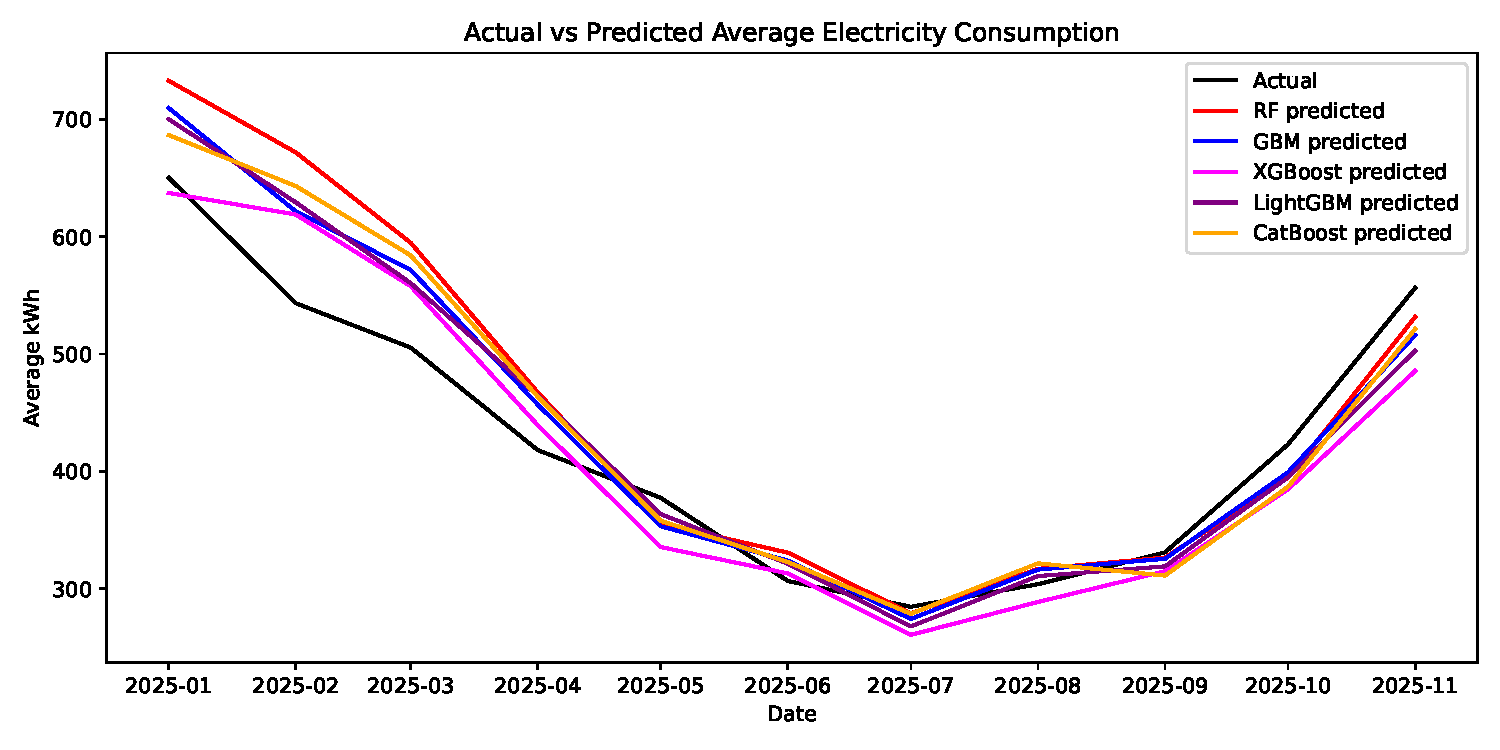
\includegraphics[width=1\linewidth]{figures/avg_predicted_vs_actual_consumption.pdf}
    \caption{Average actual versus predicted electricity consumption for all models.}
    \label{fig:avg-actual-vs-predicted}
\end{figure}

\begin{figure}[H]
    \centering
    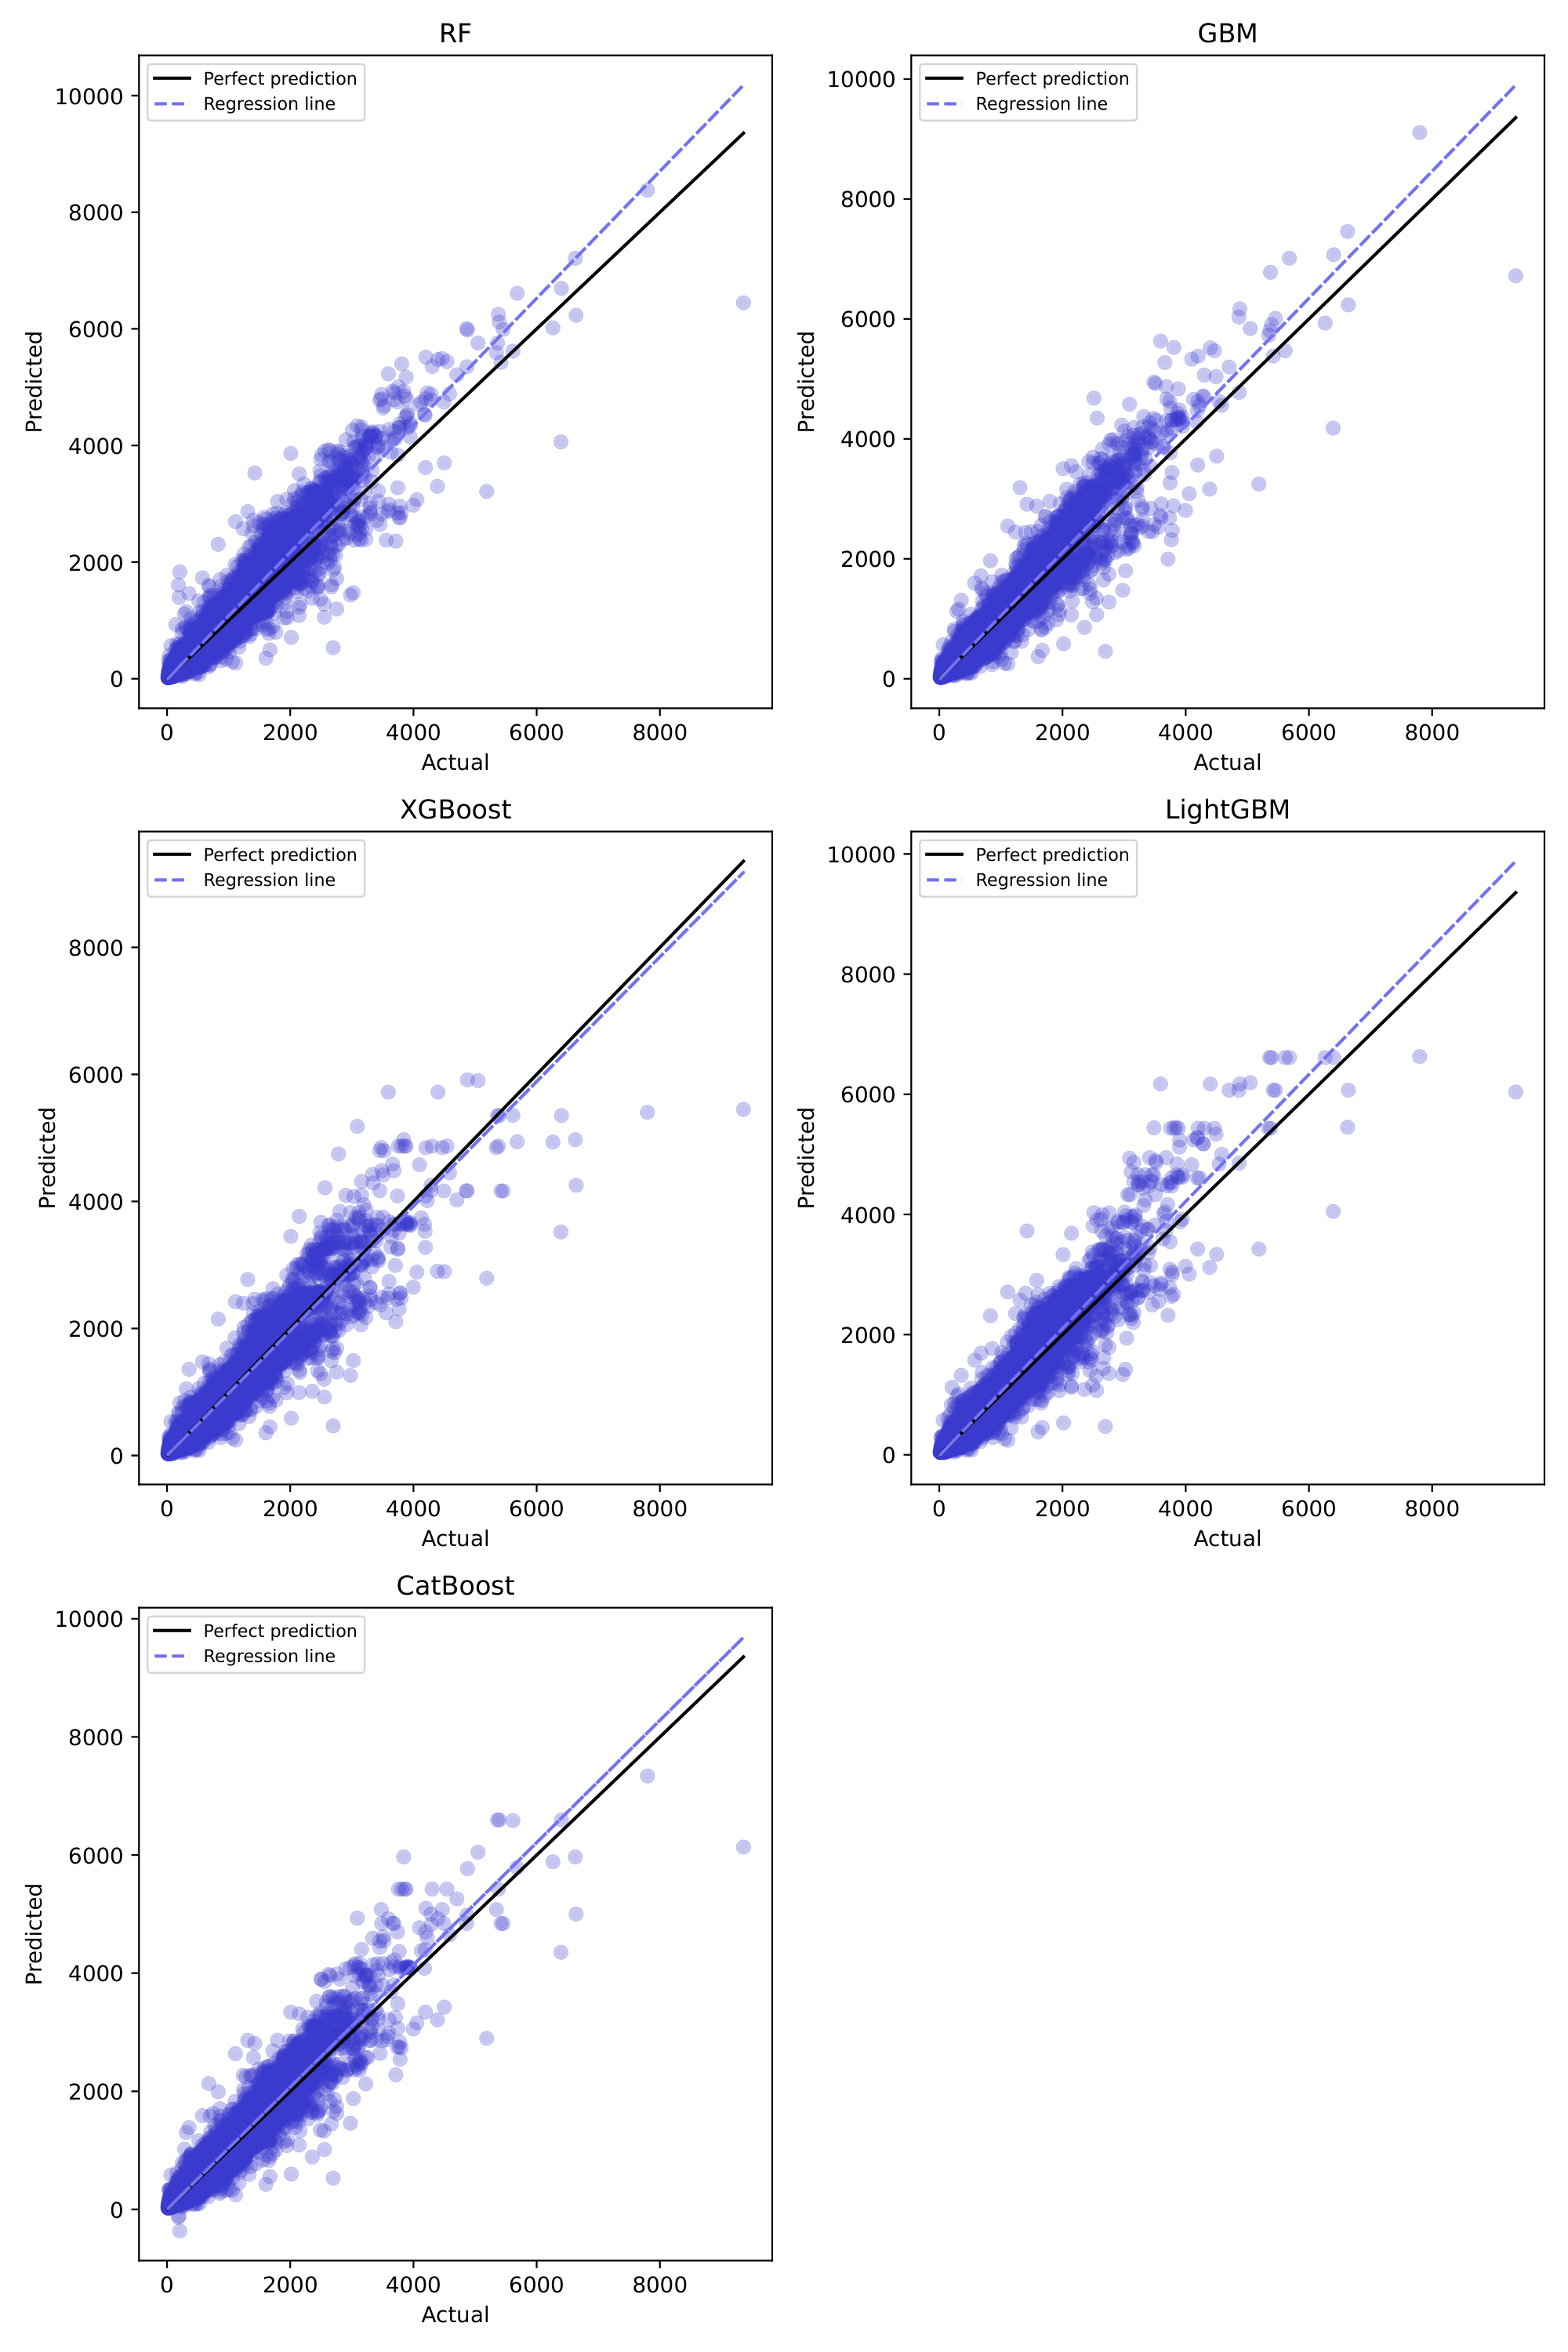
\includegraphics[width=1\linewidth]{figures/scatter_plots.png}
    \caption{Scatter plots showing prediction error distribution for each model.}
    \label{fig:scatter-plots}
\end{figure}

\subsection{Comparison with Baseline Model}

The baseline linear regression model used for comparison uses historical consumption and temperature as input variables. The past 24 months of electricity consumption and monthly average temperature was used to predict the following month's consumption. Evaluation of the linear regression model was performed using the same 2000 household sample as for the ensemble models, and the results are found in \autoref{tab:comparison-performance}. The linear regression model performs worse than the best ensemble models by roughly 3.5\% in percentage errors. RMSE and MAE scores are also worse for the linear model, especially when compared to ensemble models using only internal features.

\begin{table}[H]%[ht]
    \centering
    \caption{Performance of best ensemble model versus linear regression.}
    \label{tab:comparison-performance}
    \small
    \begin{tabularx}{\linewidth}{l r r r}
        \textbf{Model}          & \textbf{MAPE (\%)} & \textbf{RMSE (kWh)} & \textbf{MAE (kWh)} \\
        \midrule
        Best ensemble (XGBoost) & 14.96              & 153.55              & 65.46              \\
        Linear regression       & 18.47              & 161.43              & 71.98              \\
    \end{tabularx}
\end{table}

\autoref{fig:avg-actual-vs-predicted-lr} shows the average predicted monthly electricity consumption for linear regression and all ensemble models. The linear regression model shows the same tendency to overestimate the consumption during the beginning of the year as the ensemble models, while also showing a pattern of underestimating the consumption during the summer.

\begin{figure}[H]
    \centering
    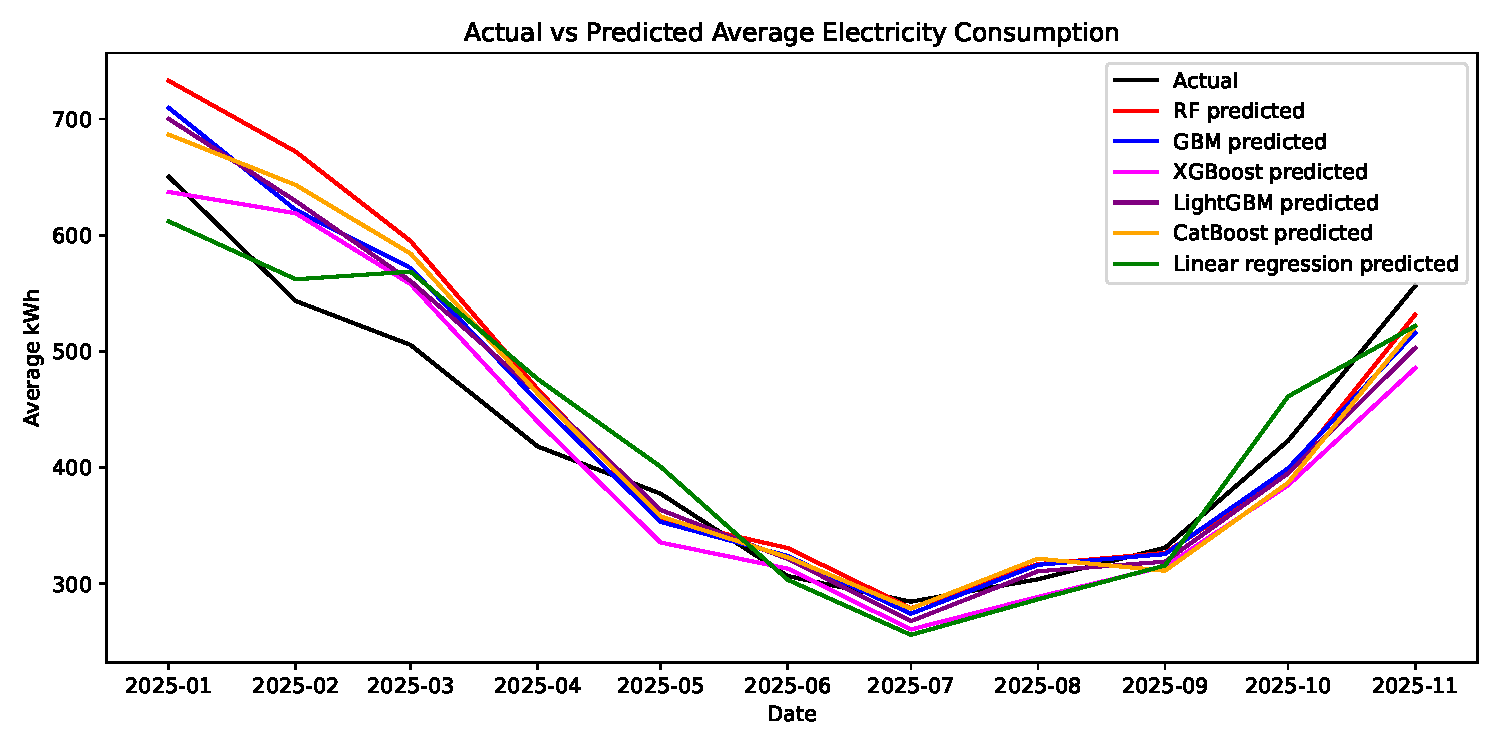
\includegraphics[width=1\linewidth]{figures/avg_predicted_vs_actual_consumption_lr.pdf}
    \caption{Average actual versus predicted electricity consumption for ensemble models and linear regression.}
    \label{fig:avg-actual-vs-predicted-lr}
\end{figure}

[maybe try LSTM and ANN for comparison too]

\section{Explainable AI Analysis of Forecasts}

All five ensemble learning models were analyzed via the SHAP method. Firstly, the models were trained using their optimal hyperparameters, and feature importance metrics were retrieved for the trained models. Secondly, a tree SHAP analysis was performed to calculate the Shapley values for all features. For the RF model, approximate SHAP values were used due to the full calculation being time-consuming for this particular model. \cref{fig:fi-shap-rf,fig:fi-shap-gbm,fig:fi-shap-xgboost,fig:fi-shap-lgbm,fig:fi-shap-catboost} show the resulting feature importance plots (left) and SHAP summary plots (right) [change to a) and b)] for each model.

Both the feature importance and SHAP analysis show that the $lag\_1$ and $lag\_12$ historical consumption features are highly influential for all models. According to the feature importance plot for GBM in \autoref{fig:fi-shap-gbm}, the model almost exclusively relies on the $lag\_1$ and $lag\_12$ features. The SHAP summary plots for all models, showing the effect of individual feature values on the prediction, also demonstrate that these features have a clear relationship where low feature values contribute to a lower predicted value, and high feature values contribute to higher predictions. Most models prioritize the $lag\_1$ feature over $lag\_12$ in their decision-making, except for RF. The $rolling\_mean\_3$ feature is ranked relatively high for all models, but the SHAP summary plots show that the feature may have a more complex relationship to the model output in some models. For GBM, XGBoost, and LightGBM, high values of the $rolling\_mean\_3$ feature contribute both to decreasing and increasing predicted values. The XGBoost model deviates from the other models by ranking the $WCT$ feature the highest in feature importance. However, the more detailed SHAP summary plot ranks the $lag\_1$ and $lag\_12$ as most influential, displaying them with a similar pattern to the other model. The SHAP summary also has a significantly lower ranking of the $WCT$ feature.

Household information features specifying residence type, and heating system were influential for the RF model, but remaining models were not as impacted by these features. The contract type feature was ranked low for all models. Even though these features commonly saw low rankings, the SHAP summaries indicate patterns where the features values had consistent impact on the SHAP values. Because of the special categorical feature handling of the CatBoost model, the SHAP summary in \autoref{fig:fi-shap-catboost} is unable to display the high/low feature value indications for these features, but it is evident that some instances of the $contract\_type$ feature had a large impact on the resulting SHAP value. In addition to the household information features, clustering of the households was performed based on their electricity consumption. The three resulting consumption groups were encoded by the $cluster$ feature. This feature was found in the lower ranks for all models.

Among the external variables, wind direction and sunshine amount are consistently ranked highly for all models. One commonly low ranked feature is the lowest cloud base feature, while remaining weather variables had a more varied impact depending on the model. The calculated weather indices $THI$ and $WCT$ also had a varied impact on the models. This can partly be attributed to the fact that the features are fully correlated with each other and with some of the weather variables [discussion probably]. The two calendar information features, $number\_of\_holidays$ and $number\_of\_days$, are commonly ranked among the less important features for the models, along with the $year$ timestamp variable. The $month$ variable, indicating the month of the year, is however ranked highly for several models.

\begin{figure}[H]
    \centering
    \makebox[\linewidth][c]{%
        \hspace{-1.5cm}
        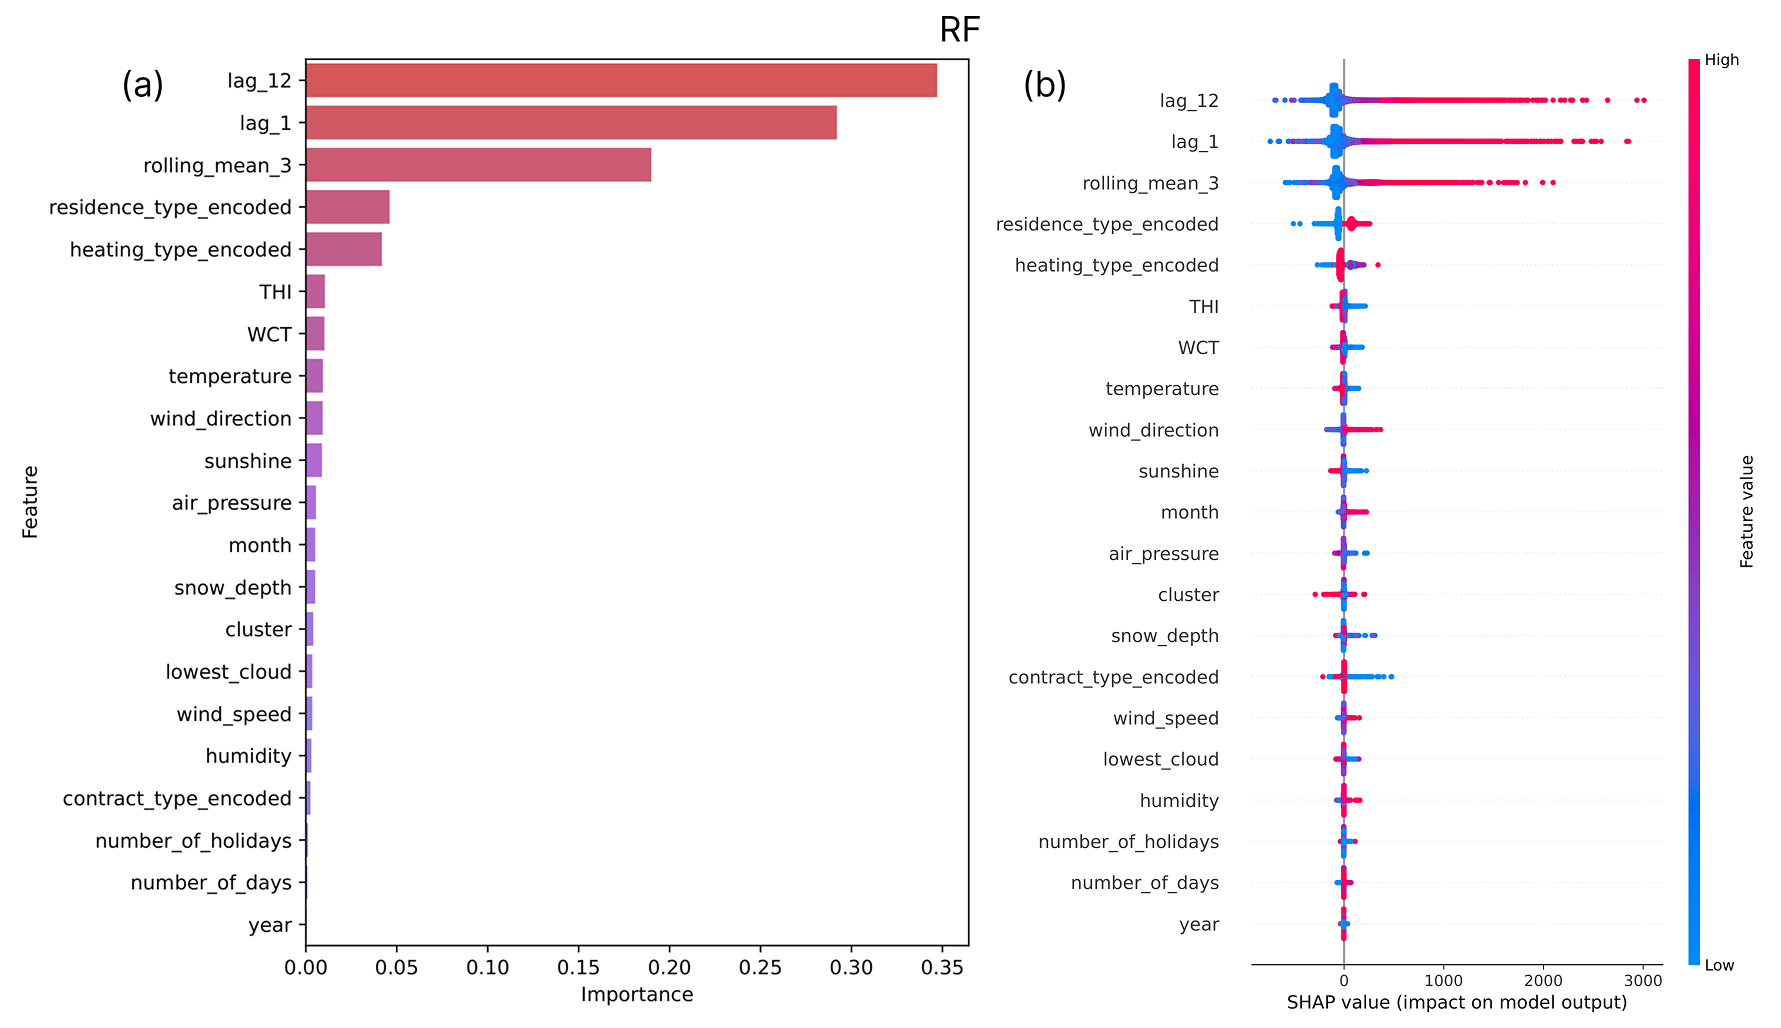
\includegraphics[width=1.25\linewidth]{figures/fi_shap_rf.png}
    }
    \caption{Feature importance and SHAP summary for RF.}
    \label{fig:fi-shap-rf}
\end{figure}

\begin{figure}[H]
    \centering
    \makebox[\linewidth][c]{%
        \hspace{-1.5cm}
        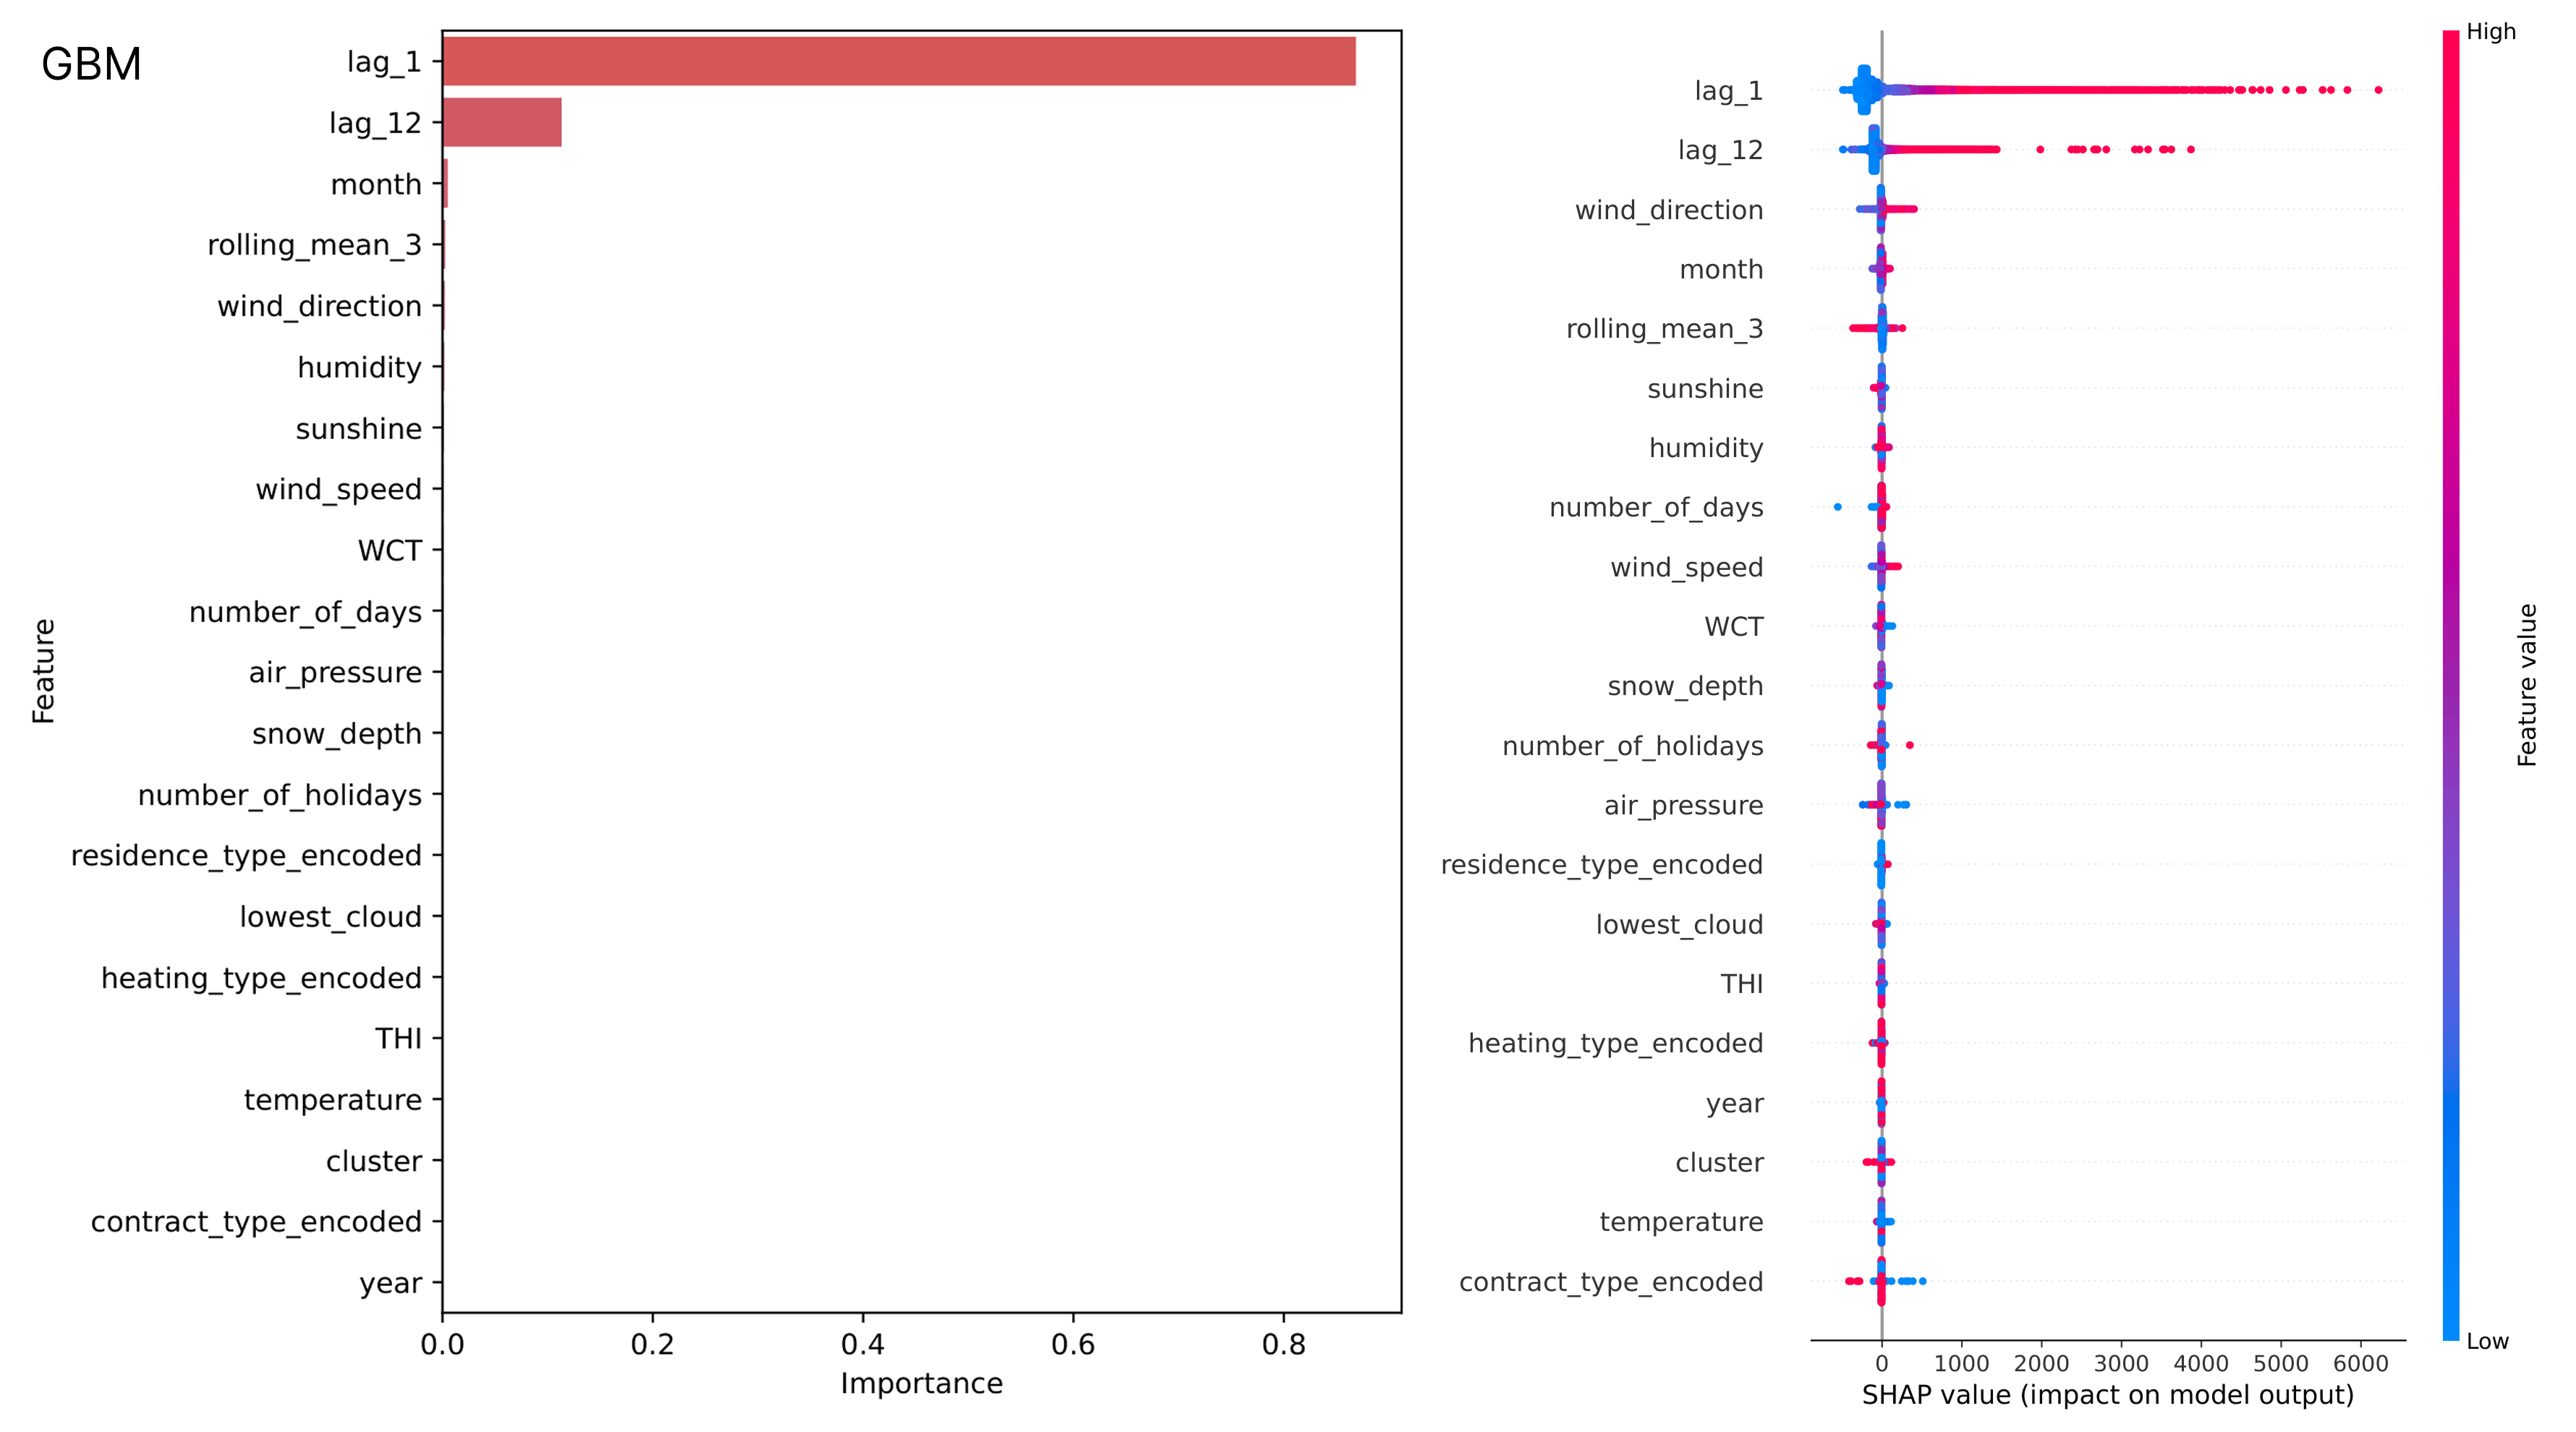
\includegraphics[width=1.25\linewidth]{figures/fi_shap_gbm.png}
    }
    \caption{Feature importance and SHAP summary for GBM.}
    \label{fig:fi-shap-gbm}
\end{figure}

\begin{figure}[H]
    \centering
    \makebox[\linewidth][c]{%
        \hspace{-1.5cm}
        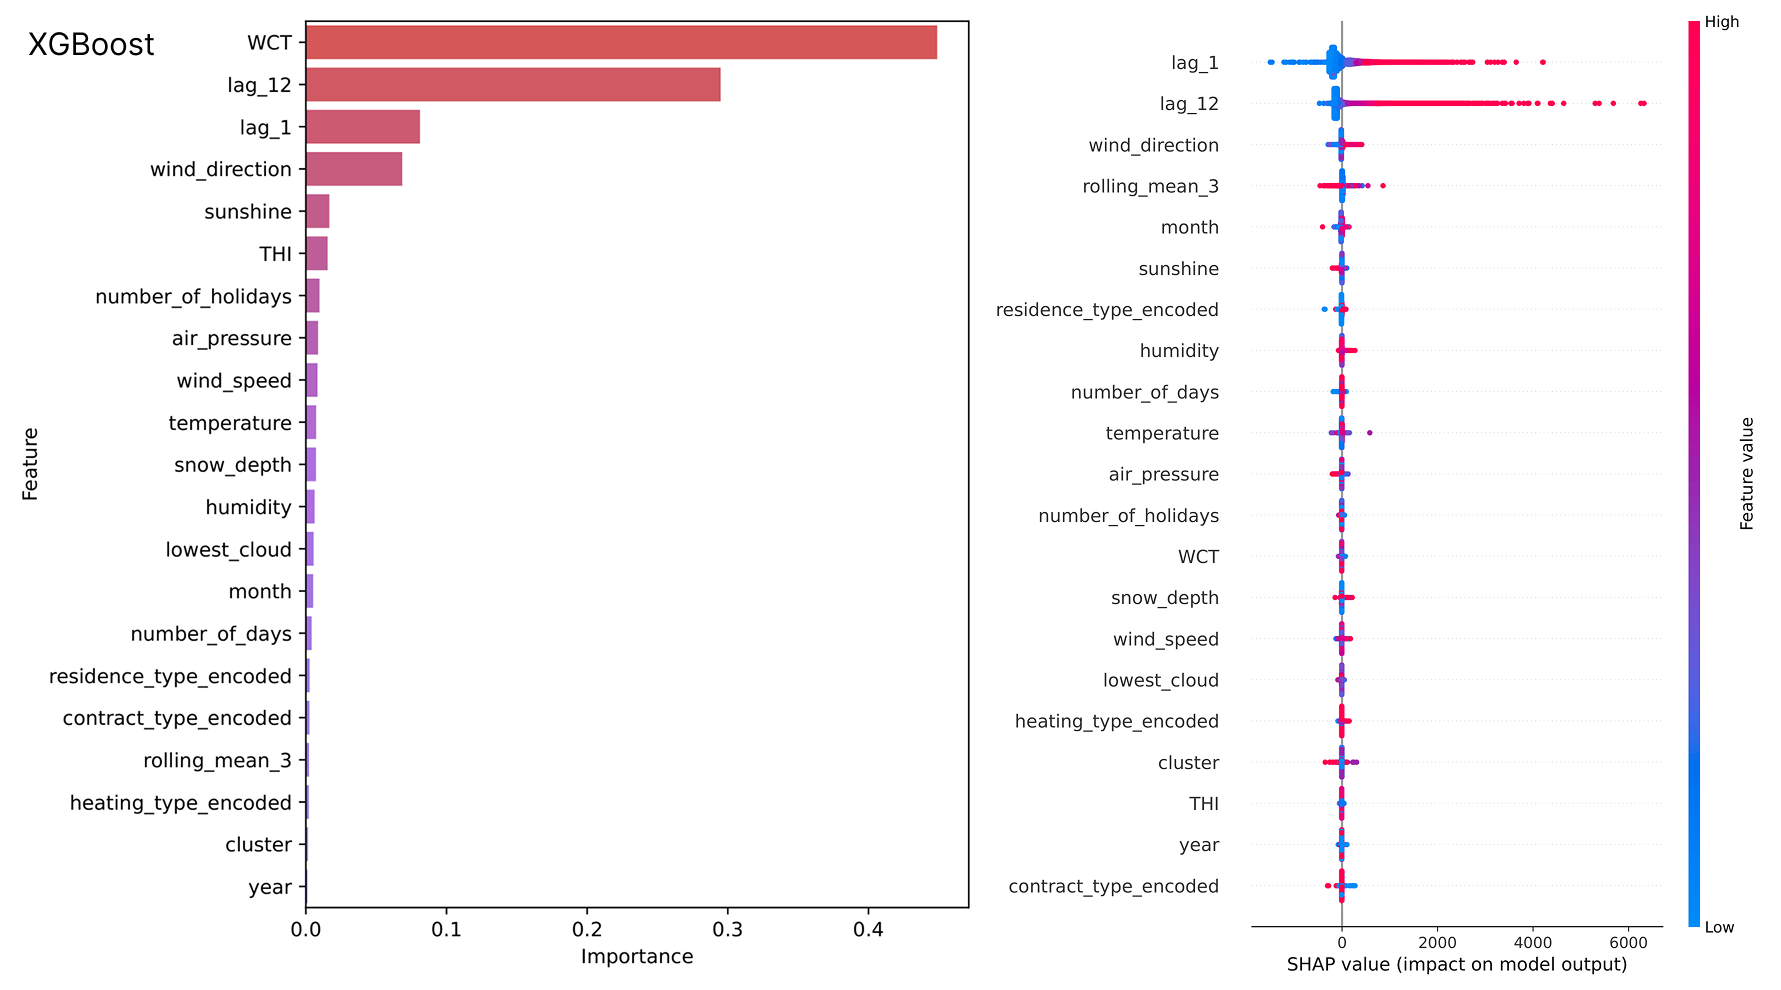
\includegraphics[width=1.25\linewidth]{figures/fi_shap_xgboost.png}
    }
    \caption{Feature importance and SHAP summary for XGBoost.}
    \label{fig:fi-shap-xgboost}
\end{figure}

\begin{figure}[H]
    \centering
    \makebox[\linewidth][c]{%
        \hspace{-1.5cm}
        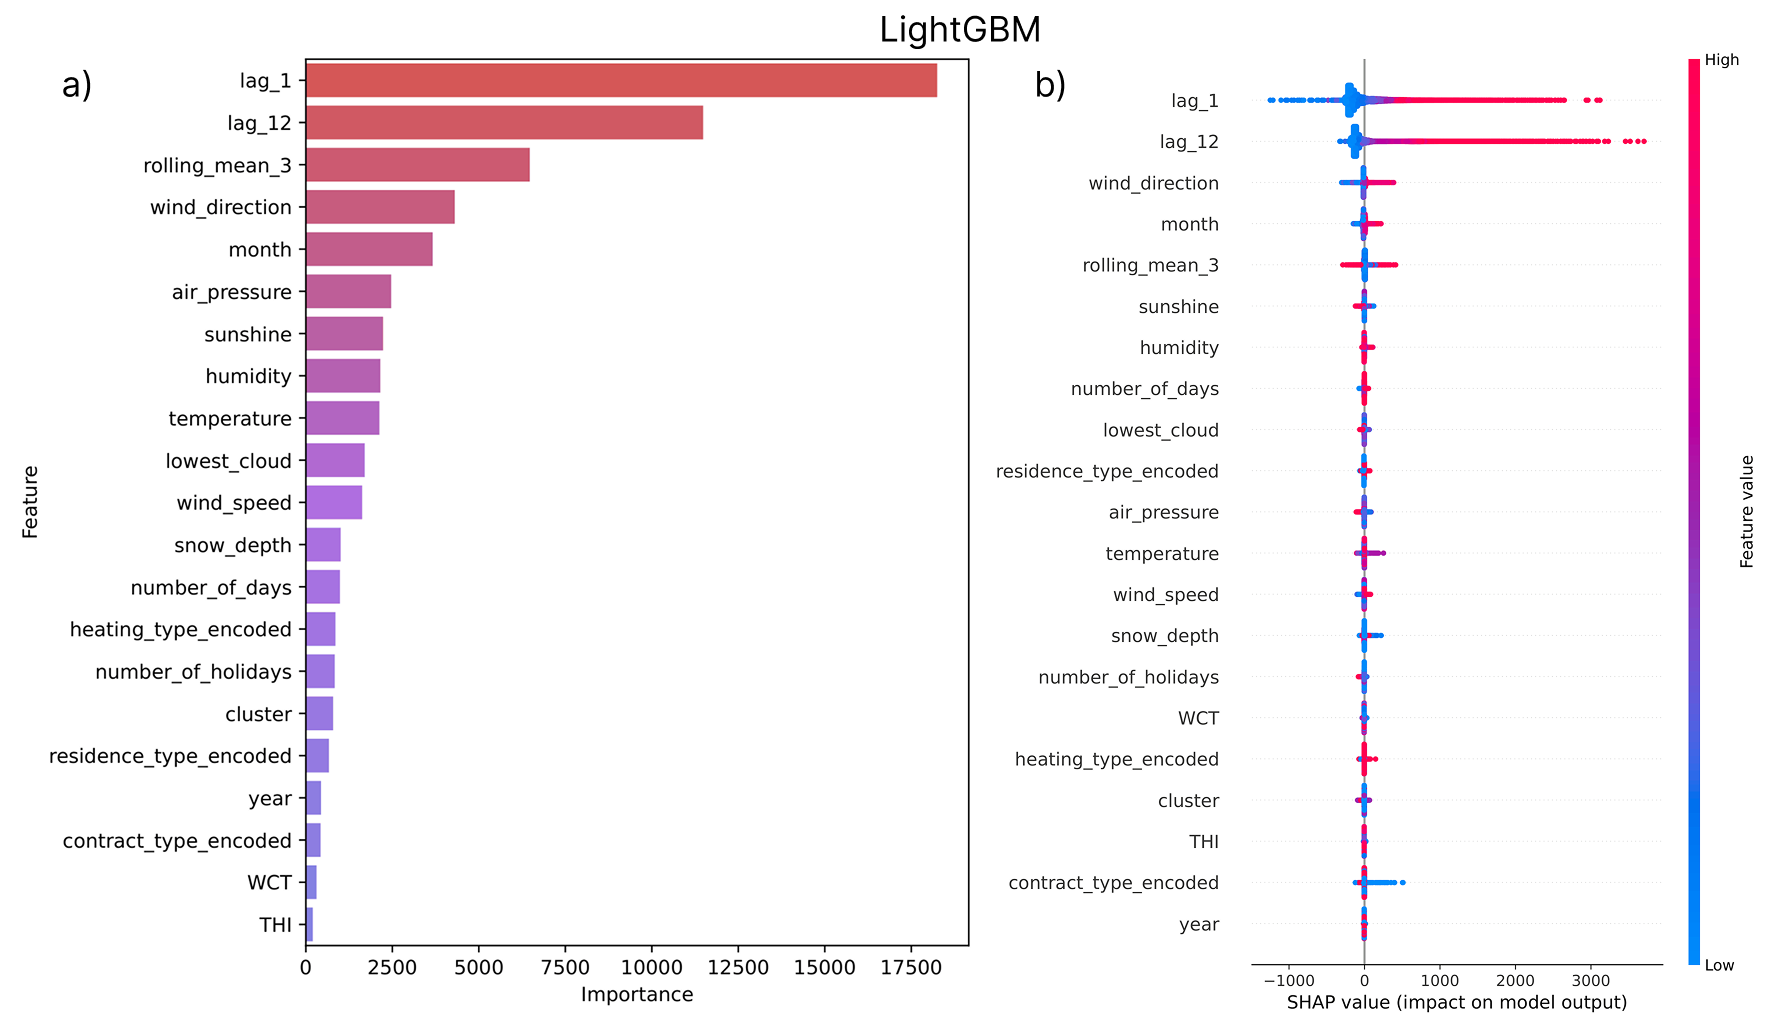
\includegraphics[width=1.25\linewidth]{figures/fi_shap_lgbm.png}
    }
    \caption{Feature importance and SHAP summary for LightGBM.}
    \label{fig:fi-shap-lgbm}
\end{figure}

\begin{figure}[H]
    \centering
    \makebox[\linewidth][c]{%
        \hspace{-1.5cm}
        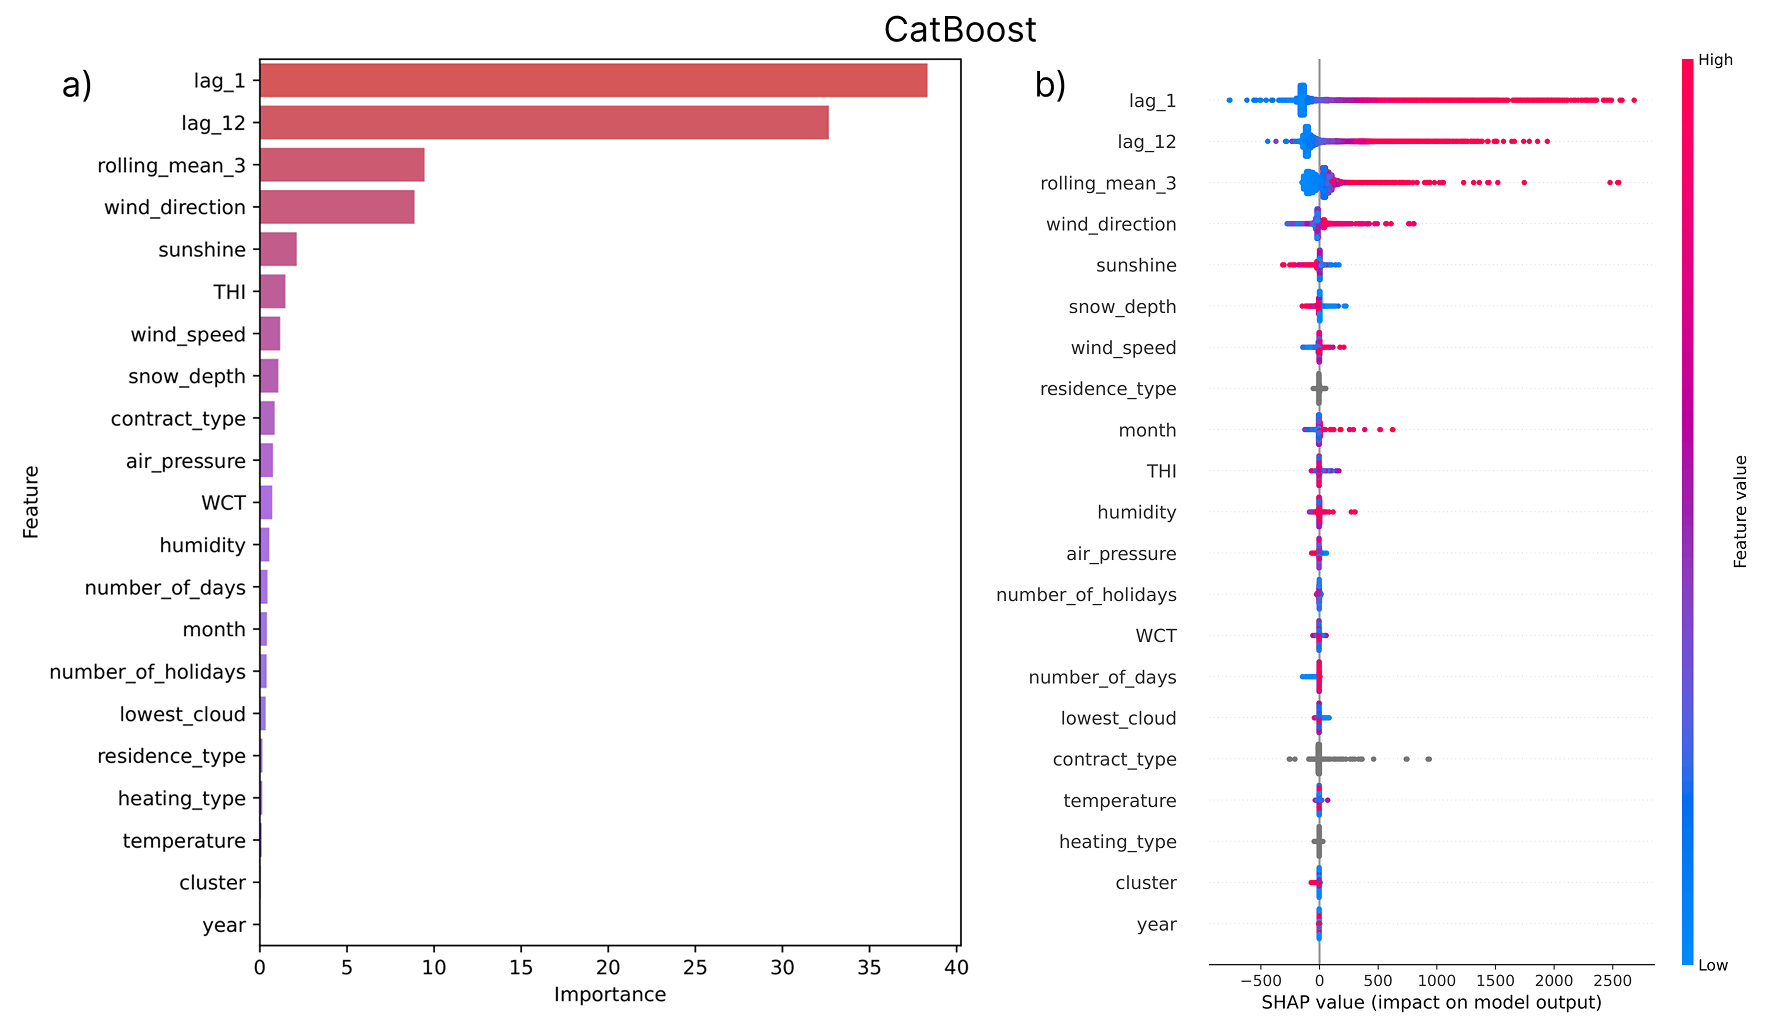
\includegraphics[width=1.25\linewidth]{figures/fi_shap_catboost.png}
    }
    \caption{Feature importance and SHAP summary for CatBoost.}
    \label{fig:fi-shap-catboost}
\end{figure}

\begin{comment}
\begin{figure}[H]
    \centering
    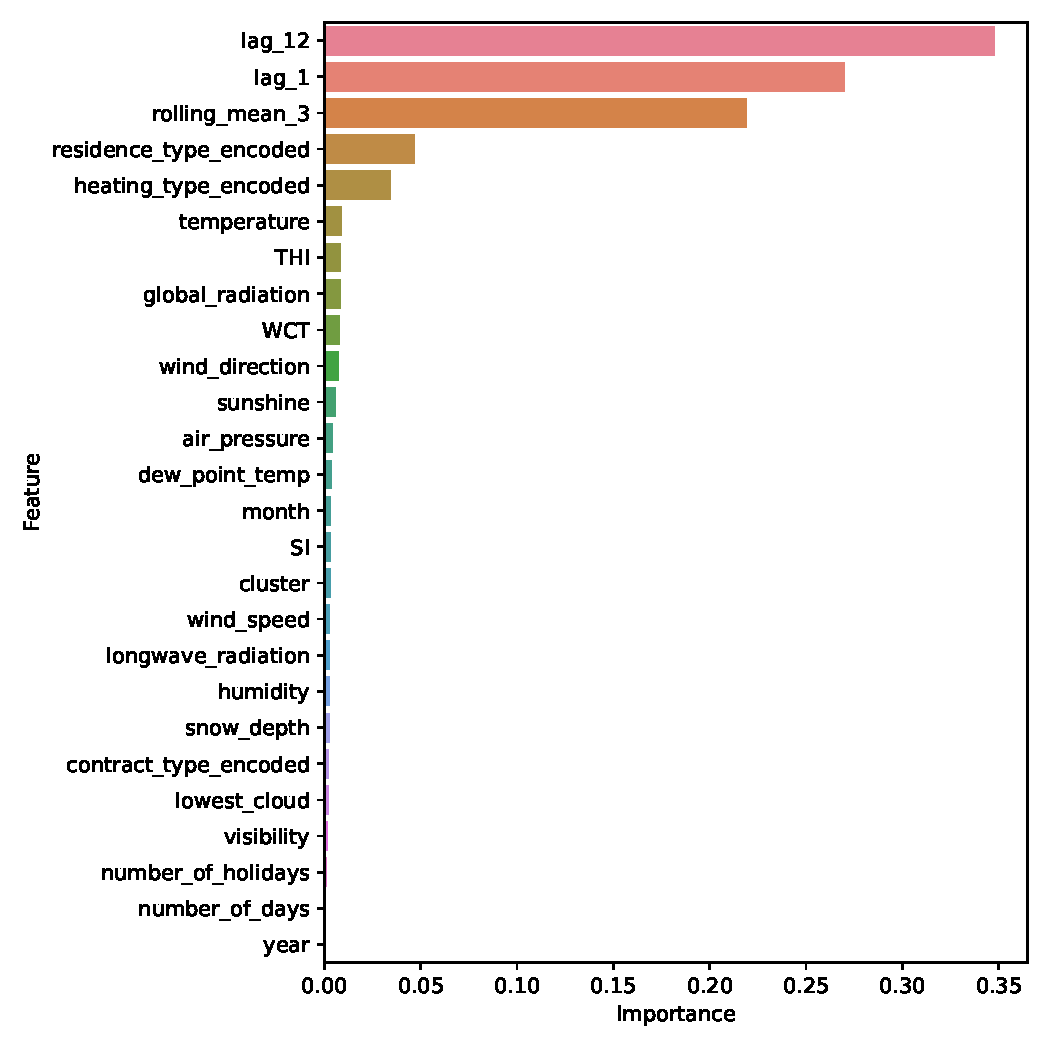
\includegraphics[width=0.9\linewidth]{figures/Fig4a_XAI_Feature_Importance_RF.pdf}
    \caption{Feature importances for RF.}
    \label{fig:feature-importances-rf}
\end{figure}

\begin{figure}[H]
    \centering
    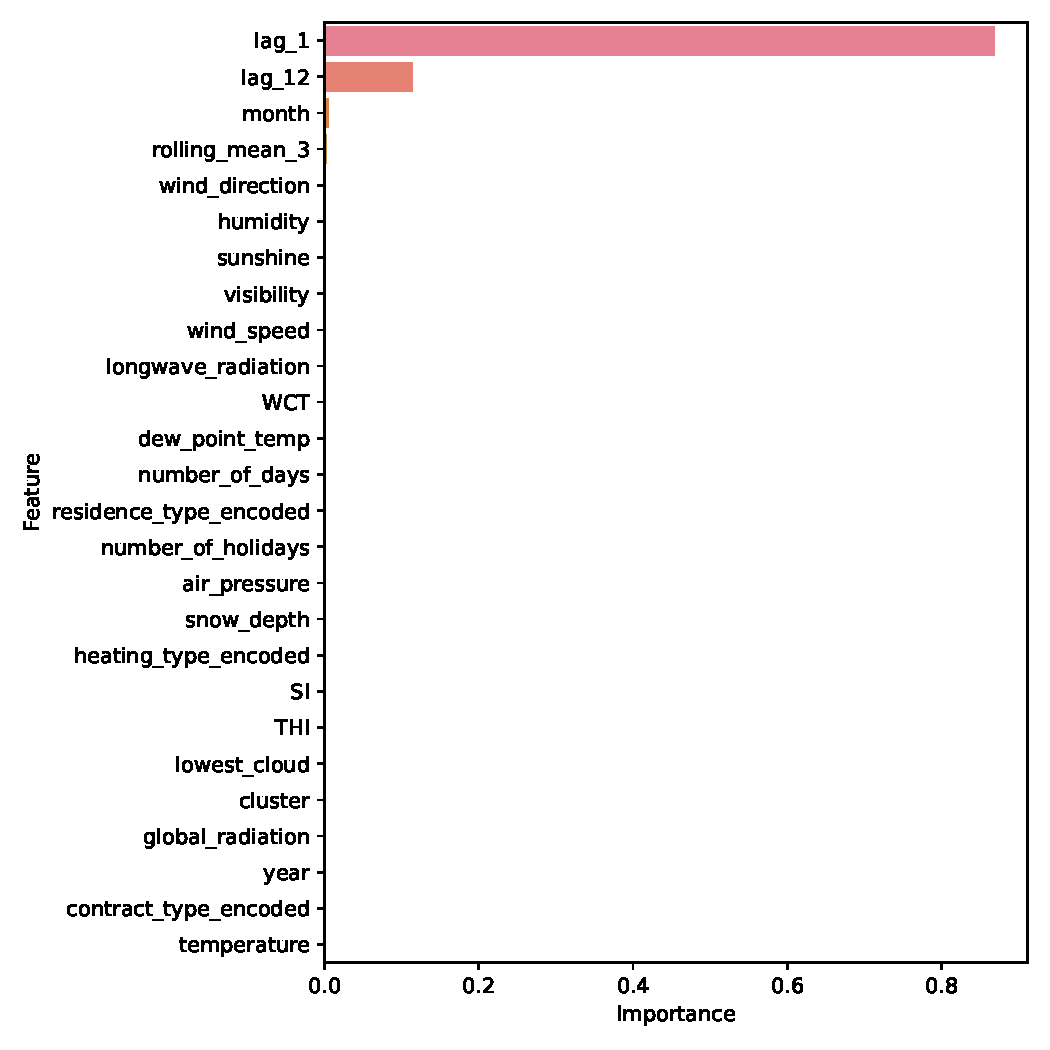
\includegraphics[width=0.9\linewidth]{figures/Fig4a_XAI_Feature_Importance_GBM.pdf}
    \caption{Feature importances for GBM.}
    \label{fig:feature-importances-gbm}
\end{figure}

\begin{figure}[H]
    \centering
    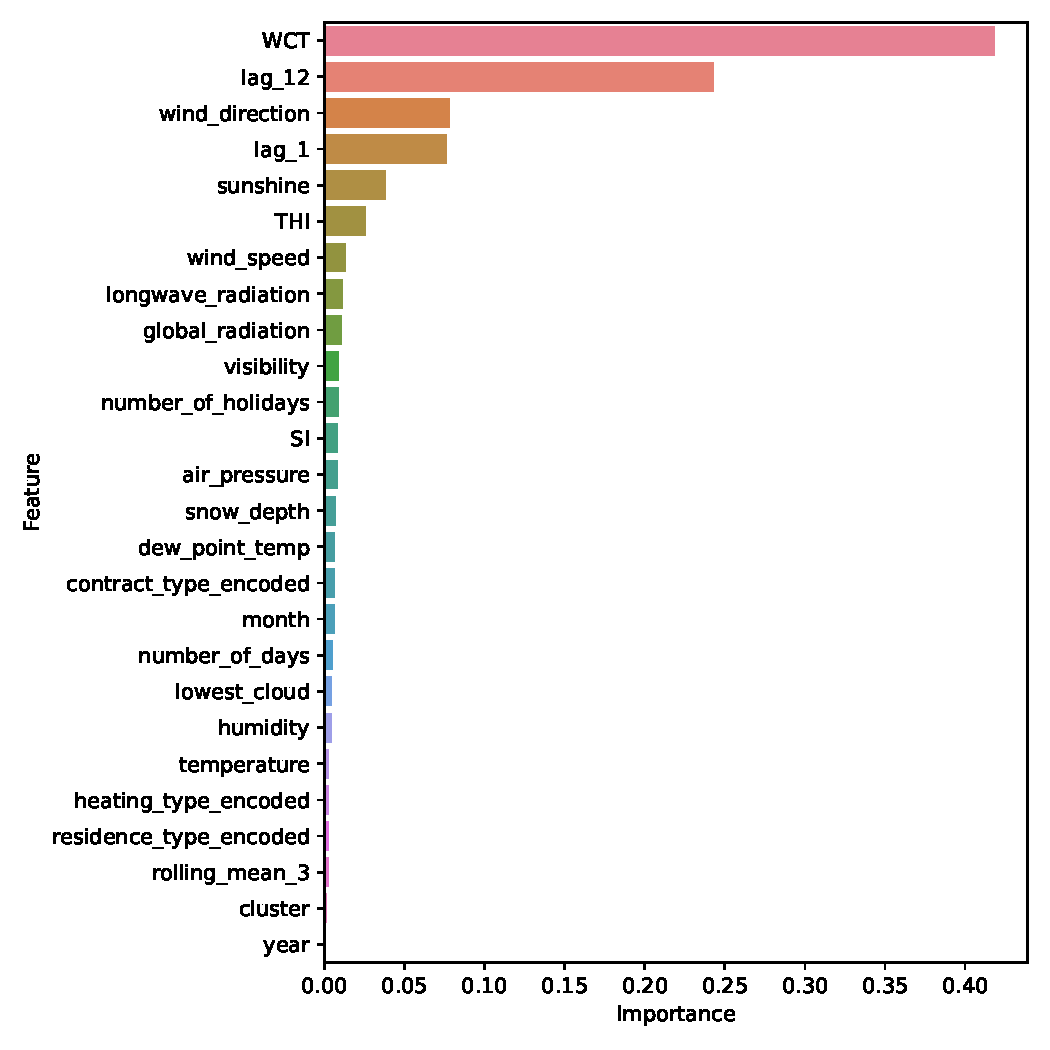
\includegraphics[width=0.9\linewidth]{figures/Fig4a_XAI_Feature_Importance_XGBoost.pdf}
    \caption{Feature importances for XGBoost.}
    \label{fig:feature-importances-xgboost}
\end{figure}

\begin{figure}[H]
    \centering
    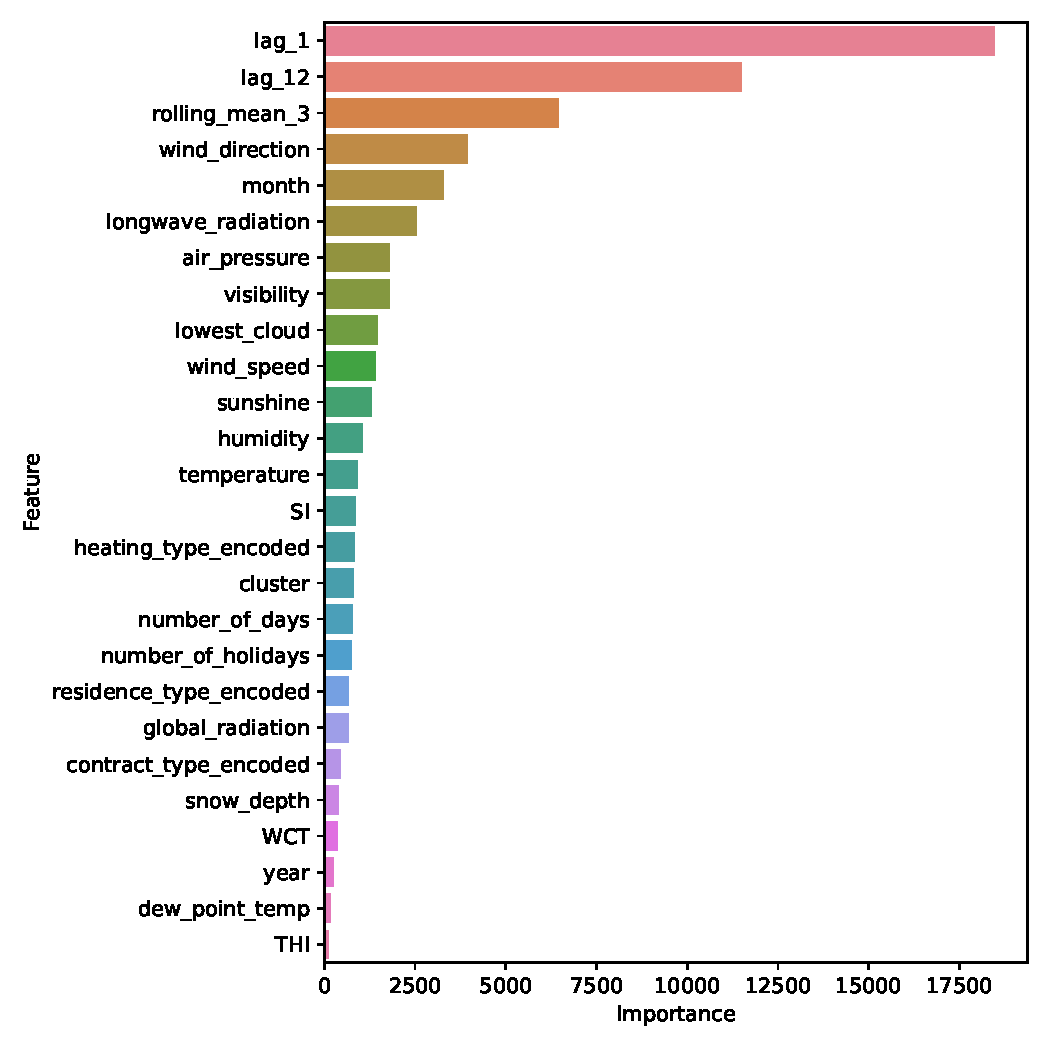
\includegraphics[width=0.9\linewidth]{figures/Fig4a_XAI_Feature_Importance_LightGBM.pdf}
    \caption{Feature importances for LightGBM.}
    \label{fig:feature-importances-lgbm}
\end{figure}

\begin{figure}[H]
    \centering
    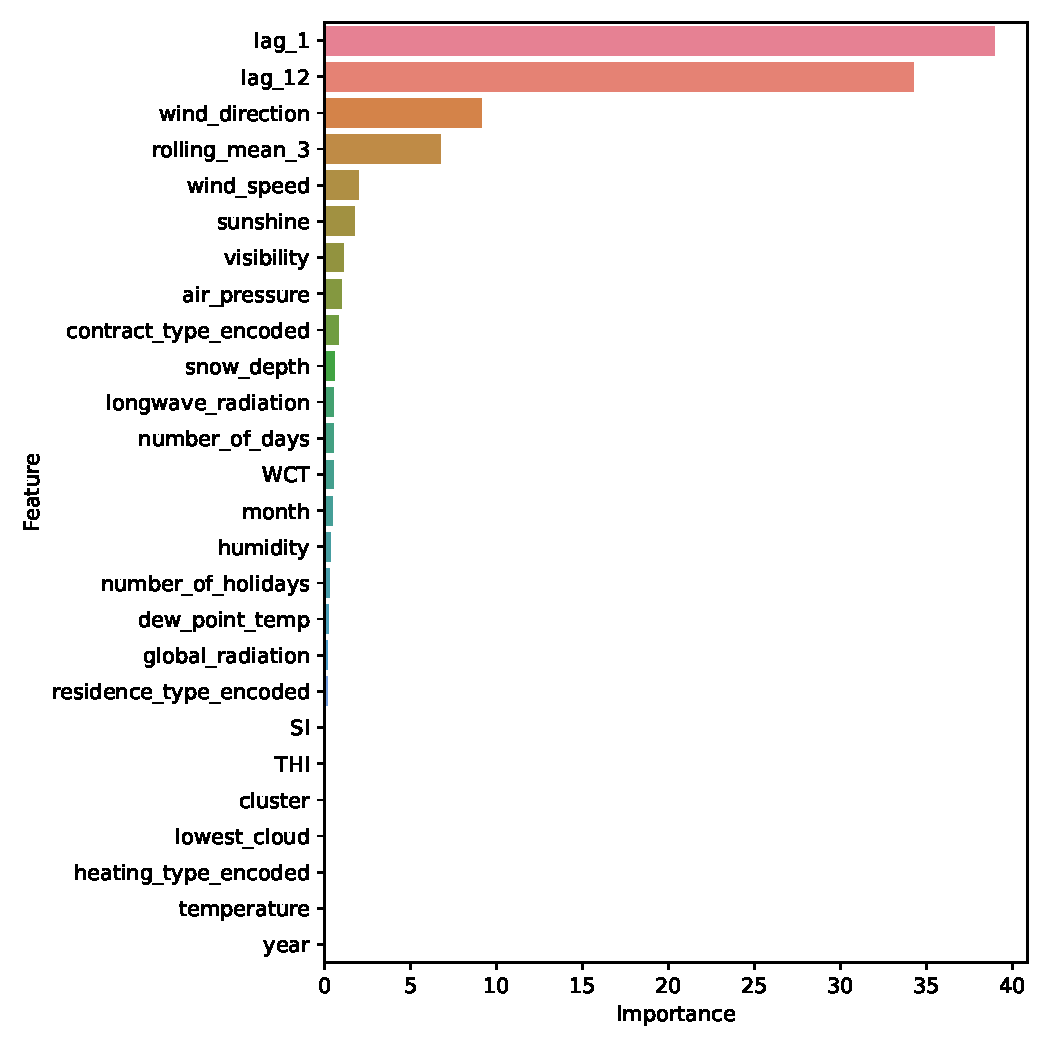
\includegraphics[width=0.9\linewidth]{figures/Fig4a_XAI_Feature_Importance_CatBoost.pdf}
    \caption{Feature importances for CatBoost.}
    \label{fig:feature-importances-catboost}
\end{figure}

\begin{figure}[H]
    \centering
    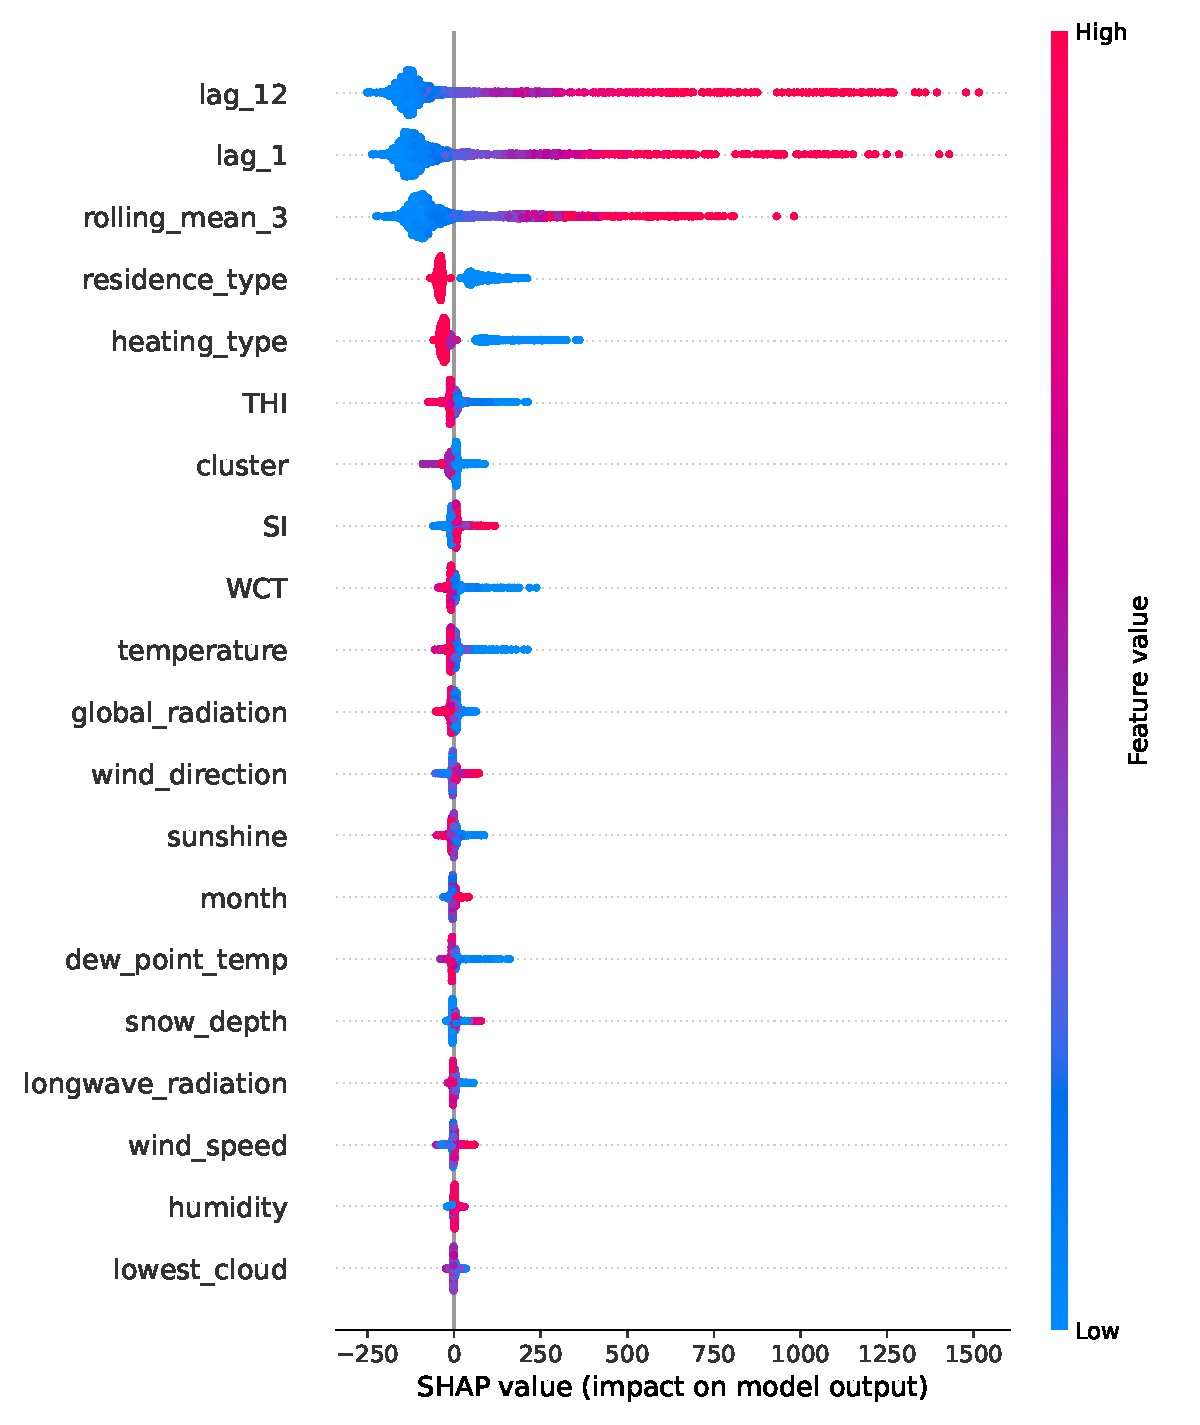
\includegraphics[width=0.9\linewidth]{figures/Fig4b_XAI_SHAP_Summary_RF.pdf}
    \caption{SHAP summary for RF [2000 sample with approximate shap values].}
    \label{fig:shap-summary-rf}
\end{figure}

\begin{figure}[H]
    \centering
    \includegraphics[width=0.9\linewidth]{figures/Fig4b_XAI_SHAP_Summary_GBM.pdf}
    \caption{SHAP summary for GBM [2000 sample].}
    \label{fig:shap-summary-gmb}
\end{figure}

\begin{figure}[H]
    \centering
    \includegraphics[width=0.9\linewidth]{figures/Fig4b_XAI_SHAP_Summary_XGBoost.pdf}
    \caption{SHAP summary for XGBoost [2000 sample].}
    \label{fig:shap-summary-xgboost}
\end{figure}

\begin{figure}[H]
    \centering
    \includegraphics[width=0.9\linewidth]{figures/Fig4b_XAI_SHAP_Summary_LightGBM.pdf}
    \caption{SHAP summary for Light GBM [2000 sample].}
    \label{fig:shap-summary-lgmb}
\end{figure}

\begin{figure}[H]
    \centering
    \includegraphics[width=0.9\linewidth]{figures/Fig4b_XAI_SHAP_Summary_CatBoost.pdf}
    \caption{SHAP summary for CatBoost [2000 sample].}
    \label{fig:shap-summary-catboost}
\end{figure}
\end{comment}

\chapter{Discussion}\label{cha:discussion}
[General introduction to discussion]

\section{Performance of Forecasting Models}

 [household energy prediction is unique because of outliers, the same problem is not prominent when predicting for an entire city e.g. future research is (probably) needed to better handle the outlier situation of household prediction, since this topic is underexplored in research]

To investigate the effect of outliers, further analysis and experiments were performed. A maximum monthly consumption threshold of 2000 kWh was selected, due to the majority of observations registering below 2000 kWh, as shown in \autoref{fig:kwh_histogram_2022_2025}. 267 households exceeding this threshold were removed from the sample of 2000 households used for the experiments. The grid search, training, and evaluation process was repeated for each model with the modified data. The resulting scores are found in \autoref{tab:performance-no-outliers}.

The removal of high-consuming households results in a small improvement in MAPE, and large improvements in both RMSE and MAE, confirming that high-consuming households have a great impact on the models' RMSE and MAE performance. The root mean squared errors were roughly half of the original for all models, and mean absolute errors decreased with around y kWh. MAPE scores improved up to 1 percentage point. Notably, the RMSE and MAE scores for the total feature group (both internal and external features) are better than for the internal group when the high-consuming households have been removed. [This suggests that external variables create noise for the households with high consumption, and actually worsen the predictive performance for this group. However, it is clear that the external variables improve the accuracy for households with a lower or medium consumption (vill förtydliga att det troligen bara är de med extremt hög konsumtion som förstör?)]

\begin{table}[H]
    \centering
    \caption{Performance of forecasting models when outlier households (i.e., households with $>$2000 kWh consumption any month) are removed from the data.}
    \label{tab:performance-no-outliers}
    \small
    \begin{tabularx}{\linewidth}{l *{6}{R}}
                       & \multicolumn{3}{c}{\textbf{Internal features}} & \multicolumn{3}{c}{\textbf{Total features}}                                                                                      \\
        \cmidrule(lr){2-4} \cmidrule(lr){5-7}
        \textbf{Model} & \textbf{MAPE (\%)}                             & \textbf{RMSE (kWh)}                         & \textbf{MAE (kWh)} & \textbf{MAPE (\%)} & \textbf{RMSE (kWh)} & \textbf{MAE (kWh)} \\
        \midrule
        RF             & 15.99                                          & 70.67                                       & 38.37              & 15.32              & 69.42               & 37.03              \\
        GBM            & 15.27                                          & 70.41                                       & 37.29              & 14.43              & 66.85               & 35.11              \\
        XGBoost        & 15.25                                          & 70.17                                       & 37.74              & 14.40              & 68.52               & 36.27              \\
        LightGBM       & 15.38                                          & 72.44                                       & 38.52              & 14.37              & 66.47               & 35.30              \\
        CatBoost       & 15.44                                          & 70.03                                       & 37.34              & 15.12              & 66.05               & 35.53              \\
        %(Linear regression) &                                                &                                             &              &               &               &              \\
    \end{tabularx}
\end{table}

\begin{figure}[H]
    \centering
    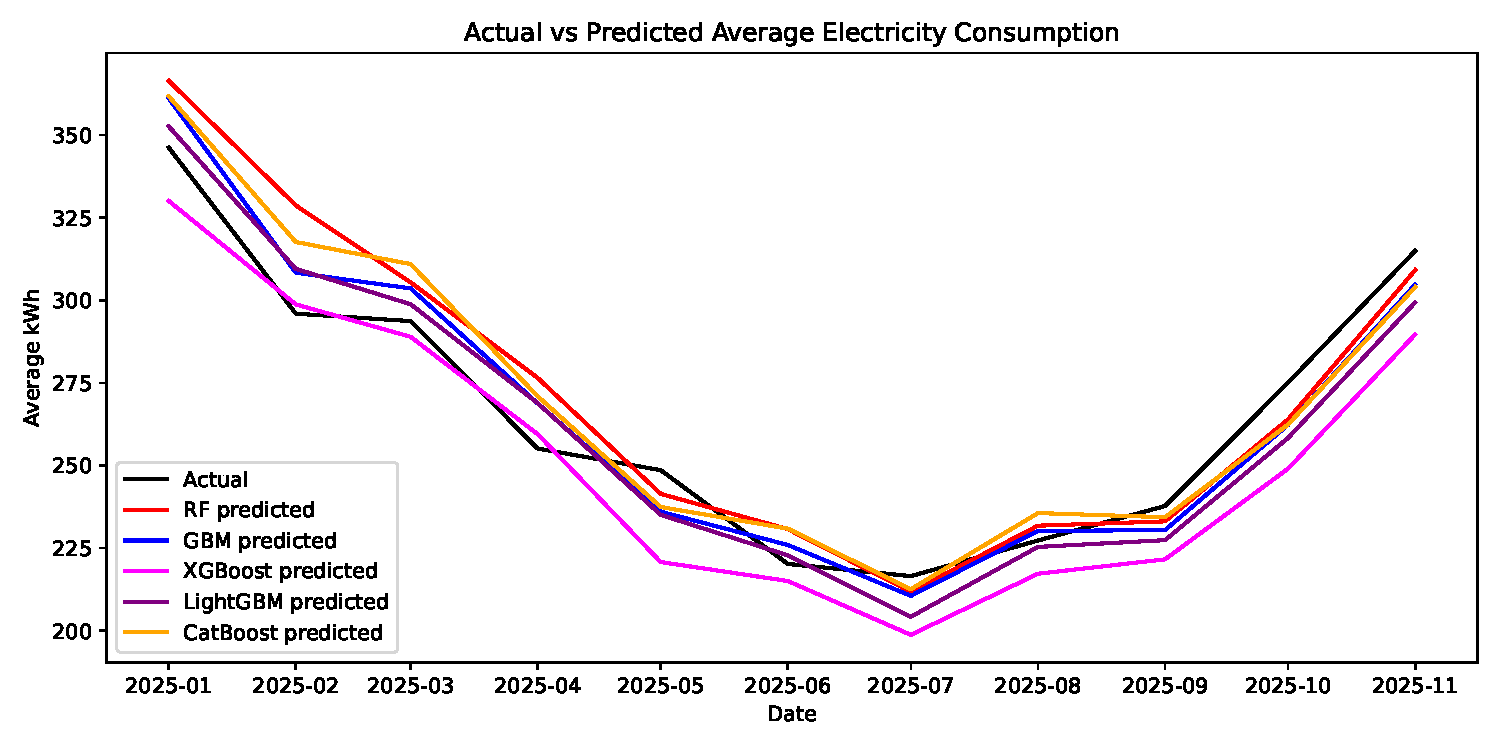
\includegraphics[width=1\linewidth]{figures/avg_predicted_vs_actual_consumption_no_outliers.pdf}
    \caption{.}
    \label{fig:avg-actual-vs-predicted-no-outliers}
\end{figure}

\begin{figure}[H]
    \centering
    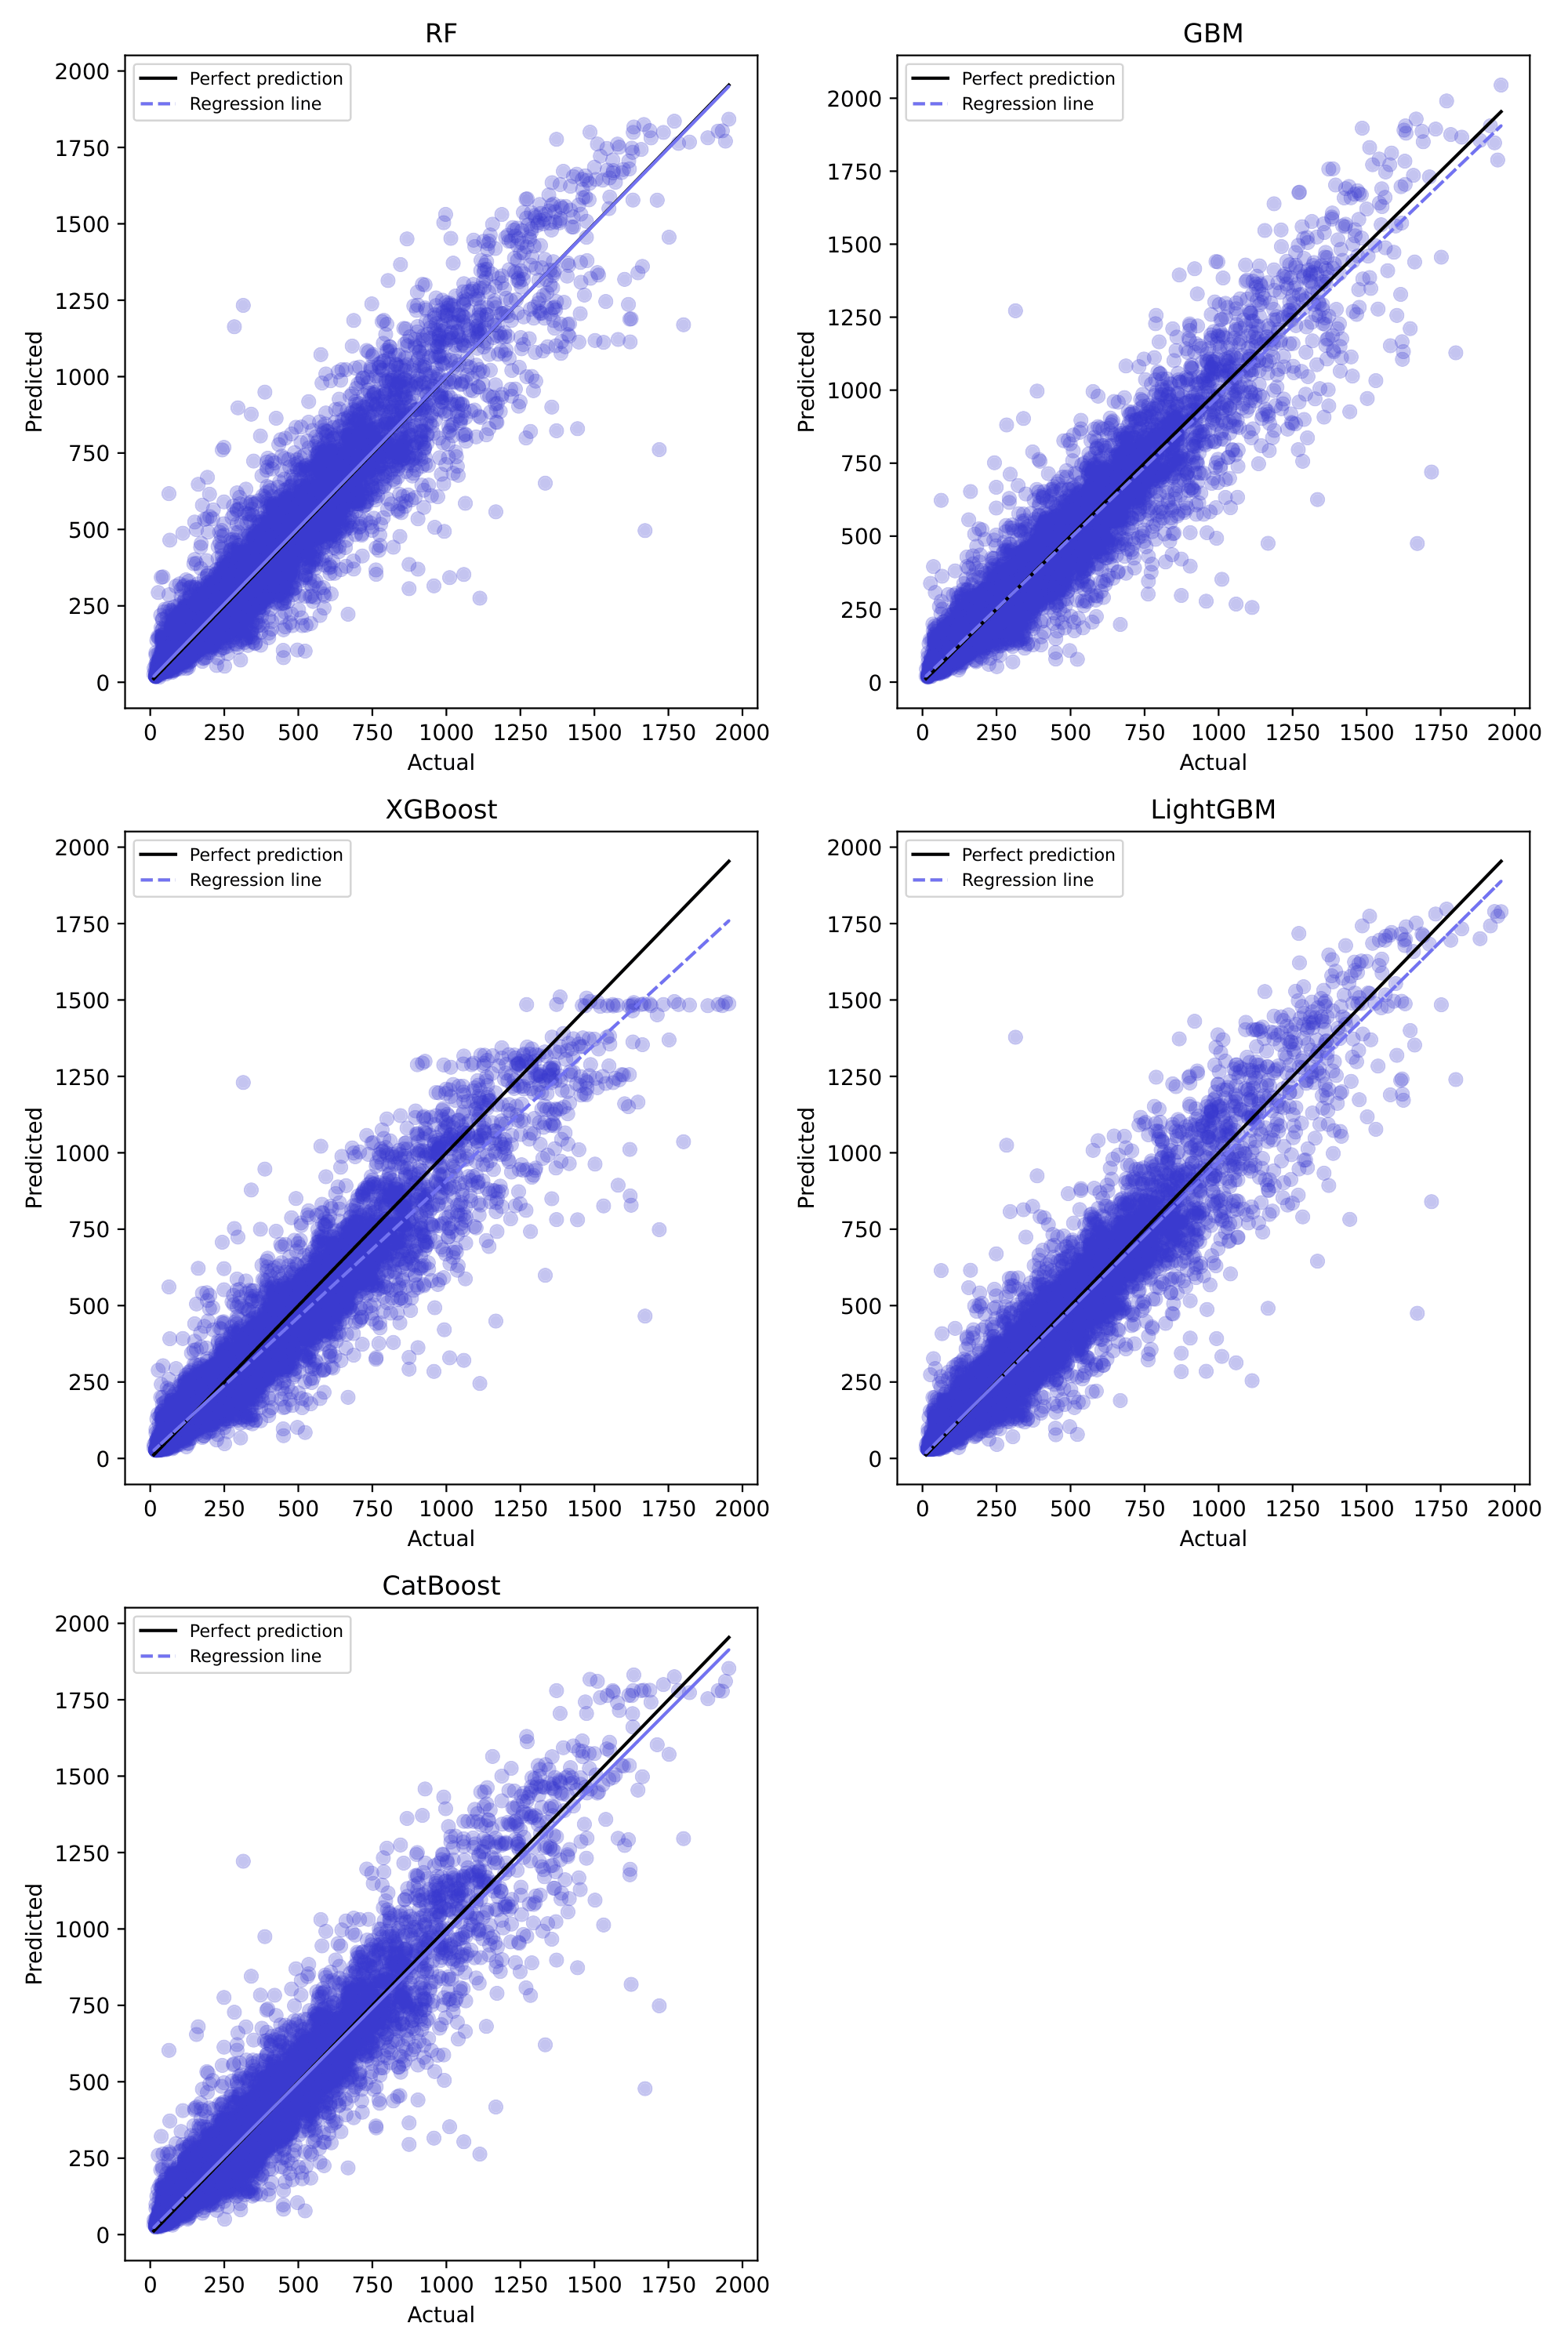
\includegraphics[width=1\linewidth]{figures/scatter_plots_no_outliers.png}
    \caption{.}
    \label{fig:scatter-plots-no-outliers}
\end{figure}

TODO: analysera mer om dessa outliers. alla bör ju ha eluppvärmning tex?

The removed households almost exclusively belonged to the house category (89\%) and vacation home category (10\%), and the majority had electrical heating (70\%).

\section{Explainable AI Forecast Analysis}
 [discuss how SHAP gives better insights than FI, XGBoost example]

The results from the XAI analysis of the forecasts provides insights into the ensemble models' decision-making, as well as perspectives on the methodologies used. A notable observation is that the simple feature importance measure did not always rank the variables' importance in the same way as the more detailed SHAP analysis. For example, the feature importance plot for XGBoost ranked $WCT$ as the most important feature, while the SHAP summary plot showed that several other variables had a more determining impact on the model's predictions.

One pattern evident in all models is that the calendar information had little impact on the forecasts. Previous works have identified holiday indicators as important for electricity consumption forecasting, since consumption patterns change between weekdays and holidays \cite{roman_holidays_2015}. Studies on short-term forecasting highlight holidays as anomalies that need to be handled in a special way, for example by introducing holidays features or by modelling holidays in a special way \cite{moon_advancing_2024,kang_off_2022,trull_one-day-ahead_2021}. However, the results in this experiment indicate that monthly forecasts are not affected by holidays in the same way as the short-term forecasts. This could be due to the effect of holidays smoothing out over the entire month, whereas in the case of e.g. day-ahead forecasting, the entire forecast would be either for a holiday or for a weekday.

    [comparisons with previous works]

\section{Limitations}

 [a big limitation is the insufficient handling of outliers, since there were many. This impacted the model performance greatly. But I just did not know what to do lol]

One limitation with this study is the method of constructing certain features, particularly external ones. All weather variables are aggregated to monthly values using mean. Some weather variables may provide more information using another aggregation method, for example, the monthly total amount of solar radiation may be a better variable than the mean solar radiation. Additionally, the process of aggregating hourly values to a single monthly value can discard valuable information. For example, Lazzari et al. \cite{lazzari_user_2022} found that minimum and maximum temperature were more important than mean temperature, possibly due to minimum and maximum temperatures having a higher variation. This indicates the existence of potential improvements by creating additional features from the weather variables than just the monthly mean. The same potential exists for the construction of more informational holiday indicators. This study only used the simple number of holidays and total number of days per month, while a better indicator could be categorizing months based on holidays.

Another limitation is the grouping of households performed via clustering. The clusters identified via the K-Means method did not show drastically different properties from each other, and the variation in electricity consumption within each cluster was high.
    [clustering was maybe not so successful. Is there a better way to divide the households into consumption groups? And how do we handle outliers in a better way?]

    [the experiments assume that all information is available. This is meant to work in a real-life scenario, where all information might not be available, for example how should new customers be handled? How should the weather data be implemented? Forecasts two weeks ahead exist, but should that be the assumption for the entire month?]

\chapter{Conclusion}\label{cha:conclusion}
This thesis investigated the novel task of enhancing interpretability of monthly electricity consumption forecasts for residential households using explainable AI. Decision tree ensemble learning models were utilized to perform the forecasts. 

[write about how household energy forecasting is special, which the main challenges were during this thesis]

[performance of model]

The performance of the five decision tree ensemble models showed similar patterns, but the best performance was exhibited by the XGBoost model. 

[write about which variables were the most important. Answer the research questions]

\section{Future Work}

[address how challenges could be handled, and what directions of research are interesting]

\begin{comment}
In some large documents, it can look nice if the first pages, with
the abstract, possible acknowledgement, table of contents, list of
figures etc. are numbered differently then the rest of the document,
usually with Roman numbers. Then the numbering restarts with the
first chapter using normal numbers. To achieve this, put
\begin{verbatim}
     \pagenumbering{roman}
\end{verbatim}
before the first page, then
\begin{verbatim}
     \cleardoublepage
     \setcounter{page}{1}
     \pagenumbering{arabic}
     \chapter{Introduction}
\end{verbatim}
before the first chapter.
\end{comment}

\cleardoublepage

%
% In order to use the bibliography{base}-command you have to prepare a "database"
% base.bib in a certain format and then run the bibtex-command (a Unix-command)
% to create a file base.bbl which LaTeX uses to create References
%
\addcontentsline{toc}{chapter}{\bibname}
\bibliographystyle{splncs}
\bibliography{main}

\appendix

\chapter{First Appendix}
\begin{figure}[H]
    \centering
    \makebox[\linewidth][c]{%
        \hspace{-1.5cm}
        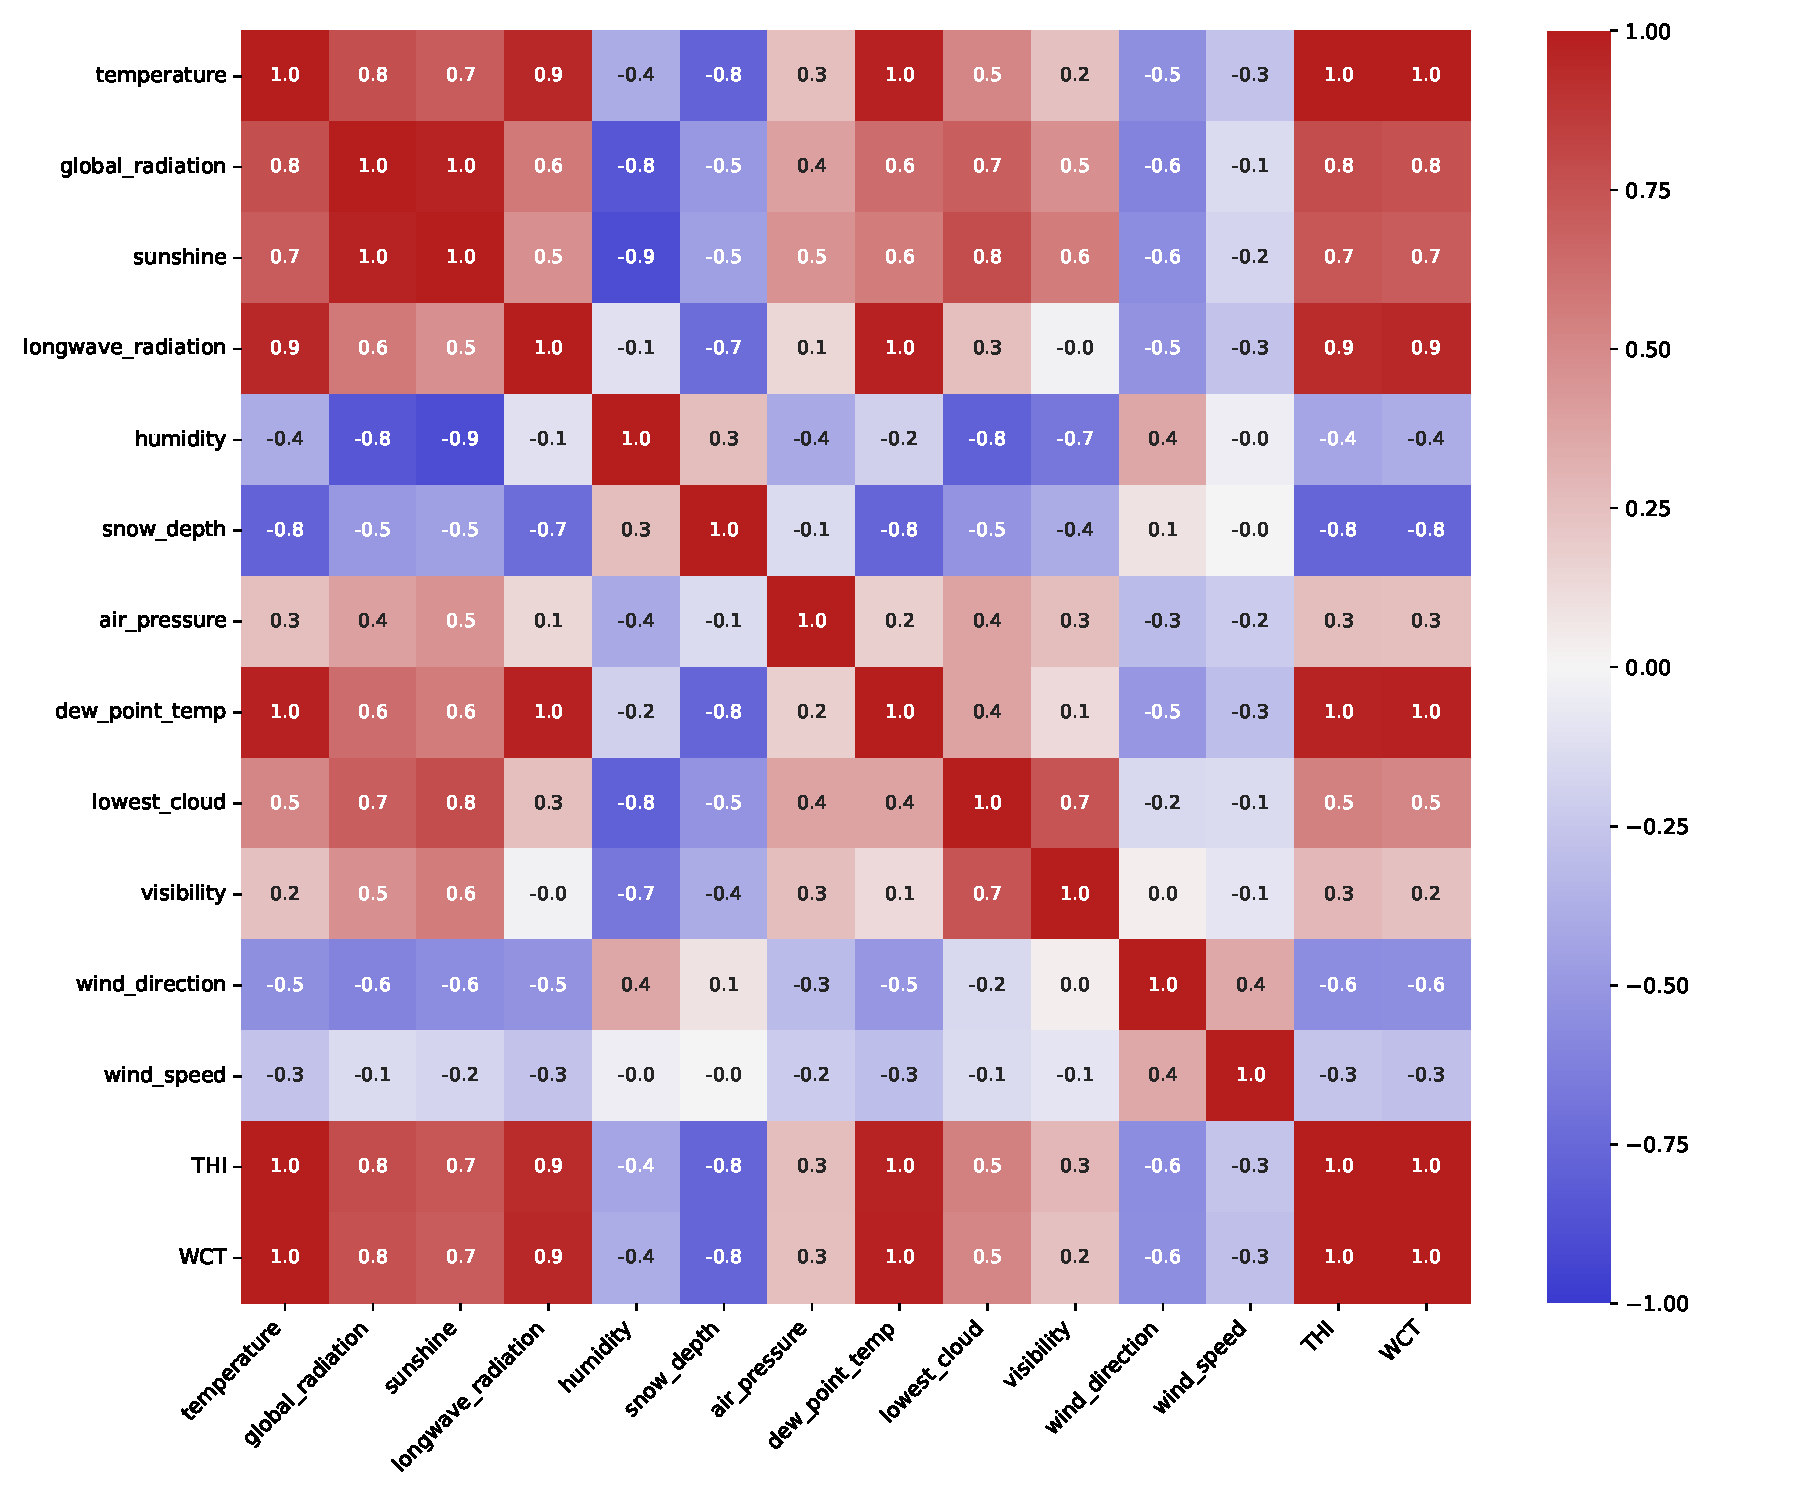
\includegraphics[width=1.2\linewidth]{figures/weather_correlation_map.pdf}
    }
    \caption{Correlation map of weather variables.}
    \label{fig:weather-correlation-map}
\end{figure}\label{cha:appendix}

\end{document}
